% 协助检查有无过期宏包及命令
\RequirePackage[l2tabu, orthodox]{nag}
% 包含beamer宏包
\documentclass[xcolor=svgnames, t]{ctexbeamer}

% 载入需要的宏包
% 加载宏包
%===================注意======================%
% 在调用beamer.cls宏包后,以下宏包将自动调用,
% 不应单独调用这些宏包,以免发生冲突
% amsfonts, amsmath, amssymb, amsthm, 
% enumerate, geometry, graphics, graphicx, 
% hyperref, url, 
% ifpdf, keyval, xcolor, xxcolor
% =============================================%
% 由于setspace宏包会改变\@footnotetext,从面造成footcite不能引用的问题,
% 以下代码用于修正这一问题
\usepackage{etoolbox}

% ++++++++++++++++++++++++++++++++++++++++++++++++++
% 为一部分代码用于解决引用setspace调整间距宏包后造成的参考文献引用脚注
% 丢失问题
\makeatletter
% save the meaning of \@footnotetext
\let\BEAMER@footnotetext\@footnotetext
\makeatother
% 调整间距
\usepackage{setspace} 
% 叉号与对号要用到的字体
\usepackage{pifont}
% 绘图
\usepackage{tikz}
\usepackage{pgfplots}
% 部分latex的Logo
\usepackage{xltxtra}
% 代码排版工具宏包
% 需要预先安装 python 和 pygments。
% 此宏包要加  -shell-escape 编译参数
% 版本2.0,支持行内代码排版
\usepackage{minted}

\usepackage{fontawesome5}

%%% Local Variables: 
%%% mode: latex
%%% TeX-master: "../main.tex"
%%% End:


% 进行必要的设置
\makeatletter
\@namedef{ver@beamerfontthememetropolis.sty}{9999/99/99}
\makeatother
\usetheme[
%%% 外部主题选项
%    hidetitle,           % 隐藏边栏中的短标题
%    hideauthor,          % 隐藏边栏中的作者缩写
%    hideinstitute,       % 隐藏边栏底部的单位缩写
%    shownavsym,          % 显示导航符号
    width=1.8cm,           % 边栏宽度 (默认是 2 cm)
%    hideothersubsections,% 除了当前section的subsection隐藏其它所有 subsections
%    hideallsubsections,  % 隐藏所有 subsections
    left,               % 边栏位置 (默认在右边)
%%% 颜色主题选项
    %lightheaderbg       % 页眉背景颜色
  ]{NWSUAFsidebar}
  
% 设置字体(参考曾祥东的latex-talk.tex进行设置)
%\usefonttheme{serif,professionalfonts}
\usefonttheme{serif,professionalfonts}
  
% Beamer settings
%\metroset{progressbar=none}
\setbeamerfont{title}{size=\huge, series=\bfseries}
\setbeamerfont*{subtitle}{size=\large, shape=\itshape}
\setbeamerfont{section title}{size=\Large, series=\bfseries}
\setbeamerfont{frametitle}{size=\large, series=\bfseries}
\setbeamerfont{caption}{size=\footnotesize, series=\bfseries}
\setbeamerfont{footnote}{size=\tiny}
\setbeamerfont{alerted text}{series=\bfseries}
%\setbeamertemplate{frame numbering}{\zhnumber[style=Financial]{\insertframenumber}}
\setbeamertemplate{itemize/enumerate subbody begin}{\footnotesize}
\setbeamertemplate{caption}{\parbox{\textwidth}{\centering\insertcaption}\par}
\setbeamertemplate{bibliography item}[text]

% PDF bookmark
\makeatletter
\apptocmd{\beamer@@frametitle}{%
  \only<1>{\expandafter\ifnum\insertcontinuationcount<2\relax
    \bookmark[page=\the\c@page,level=4]{#1}\fi}}{}{}
\makeatother


% 加载字体
% Fonts
\setmainfont{LibertinusSerif}[
  Extension      = .otf,
  UprightFont    = *-Regular,
  BoldFont       = *-Bold,
  ItalicFont     = *-Italic,
  BoldItalicFont = *-BoldItalic,
  Scale          = 1.1]
\setmonofont{Iosevka}[Scale=0.96]
\setmathfont{LibertinusMath-Regular.otf}
\setCJKmainfont{Source Han Serif SC}[
  UprightFont     = * SemiBold,
  BoldFont        = * Heavy,
  ItalicFont      = * SemiBold,
  BoldItalicFont  = * SemiBold,
  RawFeature      = +fwid]
\setCJKmonofont{Sarasa Mono SC}
  
% 部分颜色定义  
\definecolor{Descitem}{RGB}{0, 0, 139}
\definecolor{StdTitle}{RGB}{26, 33, 141}
\definecolor{StdBody}{RGB}{213,24,0}
\definecolor{AlTitle}{RGB}{255, 190, 190}
\definecolor{AlBody}{RGB}{213,24,0}
\definecolor{ExTitle}{RGB}{201, 217, 217}
\definecolor{ExBody}{RGB}{213,24,0}  

% 设置blocks
% Standard block
\setbeamercolor{block title}{fg = Descitem, bg = StdTitle!15!white}
\setbeamercolor{block body}{bg = StdBody!5!white}
% Alert block
\setbeamercolor{block title alerted}{bg = AlTitle}
\setbeamercolor{block body alerted}{bg = AlBody!5!white}
% Example block
\setbeamercolor{block title example}{bg = ExTitle}
\setbeamercolor{block body example}{bg = ExBody!5!white}
\setbeamerfont{block title}{size=\scriptsize}
\setbeamertemplate{blocks}[rounded][shadow=true]

% % 设置列表符号
% \setbeamertemplate{itemize
%   item}{\scriptsize\raise1.25pt\hbox{\donotcoloroutermaths \ding{42}}}%$\blacktriangleright$}}
% \setbeamertemplate{itemize
%   subitem}{\tiny\raise1.5pt\hbox{\donotcoloroutermaths \ding{43}}}%$\blacktriangleright$}}
% \setbeamertemplate{itemize
%   subsubitem}{\tiny\raise1.5pt\hbox{\donotcoloroutermaths \ding{45}}}%$\blacktriangleright$}}
% \setbeamertemplate{enumerate item}{\insertenumlabel.}
% \setbeamertemplate{enumerate subitem}{\insertenumlabel.\insertsubenumlabel}
% \setbeamertemplate{enumerate subsubitem}{\insertenumlabel.\insertsubenumlabel.\insertsubsubenumlabel}
% \setbeamertemplate{enumerate mini template}{\insertenumlabel}

% 设置minted宏包编排代码的参数及用于latex代码排版的简化命令
%\setminted{breaklines=true, breakautoindent=false}
\newmintinline{tex}{fontsize=\normalsize}
\newmintinline[texinlinett]{tex}{fontsize=\normalsize,escapeinside=||}
\newminted{tex}{fontsize=\scriptsize, bgcolor=yellow!20, frame=lines, autogobble}
\newminted[texcodett]{tex}{autogobble, fontsize=\scriptsize, bgcolor=yellow!20, frame=lines, escapeinside=||}
\newminted[shell]{sh}{autogobble,fontsize=\small,frame=lines}
\newmintedfile{tex}{bgcolor=yellow!20, fontsize=\footnotesize, frame=lines}

% 改变脚注的字号和符号
\setbeamerfont{footnote}{size=\zihao{7}}
\makeatletter
\def\@fnsymbol#1{\ensuremath{\ifcase#1\or *\or \dagger\or \ddagger\or
   \mathsection\or \mathparagraph\or \|\or **\or \dagger\dagger
   \or \ddagger\ddagger \else\@ctrerr\fi}}
\makeatother
\renewcommand{\thefootnote}{\fnsymbol{footnote}}

\DeclareRobustCommand{\nonumberfootnote}[2][]{%
  \let\thefootnote\relax
  \footnotetext#1{#2}}
% \renewcommand*\footnoterule{} % 取消脚注线

%% 自定义相关的名称宏命令
%% ==================================================
%% \newcommand{\yourcommand}[参数个数]{内容}
% 西北农林科技大学各单位名称
\newcommand{\nwsuaf}{西北农林科技大学}
\newcommand{\cie}{信息工程学院}
\newcommand{\cs}{计算机科学系}

% 定义引号命令
\newcommand{\qtmark}[1]{``#1''}%``''
% 定义带引号的加粗强调命令
\newcommand{\qtb}[1]{\qtmark{\emph{#1}}}
% 定义带引号的加粗加红强调命令
\newcommand{\qtbr}[1]{\qtmark{\emph{\alert{#1}}}}

% 自定义latex简单教程中要用到的宏命令
\newcommand\latex{{ \LaTeX}}%\fontfamily{cmr}\selectfont
\newcommand\msoffice{{\rmfamily MS Office}}
\newcommand\msofficepdf{\texorpdfstring{\msoffice{}}{MS Office}}
\newcommand\wysiwym{\textsc{WYSIWYM}---所想即所得}
\newcommand\wysiwyg{\textsc{WYSIWYG}---所见即所得}
\newcommand\pkg[1]{\texttt{#1}}

\colorlet{msofficecolour}{red!90!white}
\colorlet{latexcolour}{green!90!black}

% % 定义TeXLive的LOGO
\newcommand*\TeXLive{T\kern -.1667em\lower .5ex\hbox {E}\kern
  -.025emX\,Live}
\newcommand\tlive[1][2019]{
  \begin{tikzpicture}[x=1pt,y=1pt,inner sep=0pt,outer sep=0pt]
    \fill [tlblue] (0,0) rectangle (567,160);
    \node [white] at (29.7,33.8) [anchor=south west]
    {\scalebox{10}{\bfseries\TeXLive\~ #1}};
    \node at (388,9) [anchor=south west] {\includegraphics[width=15em]{tl-lion}};
    % \node [anchor=south west] {\includegraphics[height=16em]{logo}};
  \end{tikzpicture}%
}

% 论文模板名称符号
\newcommand{\nwafuthesis}{%
  \makebox{\rmfamily%
    N\hspace{-0.2ex}\raisebox{-0.5ex}{W}\raisebox{0.5ex}{\hspace{-0.2ex}\textsc{afu}}\hspace{0.3ex}%
    \textsc{Thesis}}}          

%% 定义自动扩展垂直间距的命令\stretchon和\stretchoff
%% ==================================================
\def\itemsymbol{$\blacktriangleright$}
\let\svpar\par
\let\svitemize\itemize
\let\svenditemize\enditemize
\let\svitem\item
\let\svcenter\center
\let\svendcenter\endcenter
\let\svcolumn\column
\let\svendcolumn\endcolumn
\def\newitem{\renewcommand\item[1][\itemsymbol]{\vfill\svitem[##1]}}%
\def\newpar{\def\par{\svpar\vfill}}%
\newcommand\stretchon{%
  \newpar%
  \renewcommand\item[1][\itemsymbol]{\svitem[##1]\newitem}%
  \renewenvironment{itemize}%
    {\svitemize}{\svenditemize\newpar\par}%
  \renewenvironment{center}%
    {\svcenter\newpar}{\svendcenter\newpar}%
  \renewenvironment{column}[2]%
    {\svcolumn{##1}\setlength{\parskip}{\columnskip}##2}%
    {\svendcolumn\vspace{\columnskip}}%
}
\newcommand\stretchoff{%
  \let\par\svpar%
  \let\item\svitem%
  \let\itemize\svitemize%
  \let\enditemize\svenditemize%
  \let\center\svcenter%
  \let\endcenter\svendcenter%
  \let\column\svcolumn%
  \let\endcolumn\svendcolumn%
}

%% 签署春秋学期日期命令
\newcommand{\tomonth}{
  \the\year 年\the\month 月
}

\newcommand{\tomonthen}{
  \ifcase\the\month
  \or January%
  \or February%
  \or March%
  \or April%
  \or May%
  \or June%
  \or July%
  \or August%
  \or September%
  \or October%
  \or November%
  \or December%
  \fi, \the\year
}

\newcommand{\tosemester}{
  \the\year 年\ 
  \ifcase\the\month
  \or 秋%
  \or 春%
  \or 春%
  \or 春%
  \or 春%
  \or 春%
  \or 春%
  \or 夏%
  \or 秋%
  \or 秋%
  \or 秋%
  \or 秋%
  \fi 
}

\newcommand{\tosemesteren}{  
  \ifcase\the\month
  \or Autumn%
  \or Spring%
  \or Spring%
  \or Spring%
  \or Spring%
  \or Spring%
  \or Summer%
  \or Autumn%
  \or Autumn%
  \or Autumn%
  \or Autumn%
  \or Autumn%
  \fi, \the\year
}

%% 分栏宽度
\newlength\columnskip
\columnskip 0pt
%% ==================================================          
          
% TiKz绘图设置
 \usetikzlibrary{arrows}
% TikZ宏包扩展
\usetikzlibrary{positioning}
% pgfplots设置
\pgfplotsset{compat=newest,compat/show suggested version=false}

%% 设置绘制目录结构的宏参数
\definecolor{folderbg}{RGB}{124,166,198}
\definecolor{folderborder}{RGB}{110,144,169}
\newlength\Size
\setlength\Size{4pt}
\tikzset{%
  folder/.pic={%
    \filldraw [draw=folderborder, top color=folderbg!50, bottom color=folderbg] (-1.05*\Size,0.2\Size+5pt) rectangle ++(.75*\Size,-0.2\Size-5pt);
    \filldraw [draw=folderborder, top color=folderbg!50, bottom color=folderbg] (-1.15*\Size,-\Size) rectangle (1.15*\Size,\Size);
  },
  file/.pic={%
    \filldraw [draw=folderborder, top color=folderbg!5, bottom color=folderbg!10] (-\Size,.4*\Size+5pt) coordinate (a) |- (\Size,-1.2*\Size) coordinate (b) -- ++(0,1.6*\Size) coordinate (c) -- ++(-5pt,5pt) coordinate (d) -- cycle (d) |- (c) ;
  },
}
\forestset{%
  declare autowrapped toks={pic me}{},
  declare boolean register={pic root},
  pic root=0,
  pic dir tree/.style={%
    for tree={%
      folder,
      %font=\ttfamily,
      grow'=0,
      s sep=1.0pt,
      font=\small \sffamily,
      %fit=band,
      %ysep = 1.0pt,
      inner ysep = 2.6pt,
    },
    before typesetting nodes={%
      for tree={%
        edge label+/.option={pic me},
      },
      if pic root={
        tikz+={
          \pic at ([xshift=\Size].west) {folder};
        },
        align={l}
      }{},
    },
  },
  pic me set/.code n args=2{%
    \forestset{%
      #1/.style={%
        inner xsep=2\Size,
        pic me={pic {#2}},
      }
    }
  },
  pic me set={directory}{folder},
  pic me set={file}{file},  
}
%% ==================================================

%%%%%%%%%%%%%%%%%%%%%%%%%%%%%%%%%%%%%%%%%%%%%%%%%%%%%%%%%%%%%%%%%%%%%%
% LaTeX Overlay Generator - Annotated Figures v0.0.2
% Created with http://ff.cx/latex-overlay-generator/
% If this generator saves you time, consider donating 5,- EUR! :-)
%%%%%%%%%%%%%%%%%%%%%%%%%%%%%%%%%%%%%%%%%%%%%%%%%%%%%%%%%%%%%%%%%%%%%%
%                         #1          #2       #3         #4           #5          #6            #7           #8
%\annotatedFigureBox{bottom-left}{top-right}{label}{label-position}{box-color}{label-color}{border-color}{text-color}
\newcommand*\annotatedFigureBoxCustom[8]{\draw[#5,thick,rounded corners] (#1) rectangle (#2);\node at (#4) [fill=#6,thick,shape=circle,draw=#7,inner sep=2pt,font=\sffamily,text=#8] {\textbf{#3}};}
\newcommand*\annotatedFigureBoxLabel[4]{\annotatedFigureBoxCustom{#1}{#2}{#3}{#4}{red}{white}{black}{black}}
\newcommand*\annotatedFigureBox[3]{\draw[#3,thick,rounded corners=0.5mm] (#1) rectangle (#2);}
\newenvironment {annotatedFigure}[1]{\centering\begin{tikzpicture}\node[anchor=south west,inner sep=0] (image) at (0,0) { #1};\begin{scope}[x={(image.south east)},y={(image.north west)}]}{\end{scope}\end{tikzpicture}}
%%%%%%%%%%%%%%%%%%%%%%%%%%%%%%%%%%%%%%%%%%%%%%%%%%%%%%%%%%%%%%%%%%%%%%

% 动态改变menukeys宏包的win/mac样式
\makeatletter
\def\setmenukeyswin{\def\tw@mk@os{win}}
\def\setmenukeysmac{\def\tw@mk@os{mac}}
\makeatother

% 插图路径设置
% ==================================================
\graphicspath{{figures/}}%图片所在的目录
% ==================================================

% 为标题页指定一个 logo
\pgfdeclareimage[height=0.8cm]{titlepagelogo}{nwsuaflogo/nwsuaf_logo_new}% 标题页
\titlegraphic{% 标题页底部
  \pgfuseimage{titlepagelogo}%
}

\newcommand\CASE[1]{{\addfontfeatures{Letters=Uppercase}#1}}
\newcommand\jatext[1]{{\addCJKfontfeatures{Language=Japanese}#1}}
\newcommand\link[1]{\href{#1}{\ \faExternalLinkSquare*}}%\faLink \faExternalLink*


% PoZheHao, see https://github.com/CTeX-org/ctex-kit/issues/382
\ExplSyntaxOn
\xeCJK_new_class:n { PoZheHao }
\__xeCJK_save_CJK_class:n { PoZheHao }
\xeCJK_declare_char_class:nn { PoZheHao } { "2014 }
\seq_map_inline:Nn \g__xeCJK_class_seq
  {
    \str_if_eq:nnF {#1} { PoZheHao }
      {
        \xeCJK_copy_inter_class_toks:nnnn { PoZheHao } {#1} { FullRight } {#1}
        \xeCJK_copy_inter_class_toks:nnnn {#1} { PoZheHao } {#1} { FullRight }
      }
  }
\ExplSyntaxOff

% Hack
% Use small caps for LaTeX symbol
\DeclareRobustCommand{\LaTeX}{%
  L\kern-.3em%
  \raisebox{.2em}{\textsc{a}}\kern-.14em%
  \TeX}
% Compatibility with unicode-math
\DeclareRobustCommand{\LaTeXe}{%
  \LaTeX\kern.15em2%
  \hbox{%
    \if b\expandafter\@car\f@series\@nil
      $_{\textstyle\symbf{\varepsilon}}$%
    \else
      $_{\textstyle\varepsilon}$%
    \fi}}  



%%% Local Variables: 
%%% mode: latex
%%% TeX-master: "../main.tex"
%%% End: 


%% 输出绘制有文档线条的笔记区
%\pgfpagesuselayout{4 on 1 with notes}[a4paper,border shrink=5mm]
%\pgfpagesuselayout{1 on 1 with notes landscape}[a4paper, border shrink=5mm]
%\pgfpagesuselayout{2 on 1 with notes}[a4paper,border shrink=5mm]
%\pgfpagesuselayout{3 on 1 with notes}[a4paper,border shrink=5mm]
%\pgfpagesuselayout{2 on 1 with notes landscape}[a4paper,border shrink=5mm]
%\pgfpagesuselayout{1 on 1 with notes}[a4paper,border shrink=5mm]

% 打开PDF后直接全屏
%\hypersetup{pdfpagemode={FullScreen}}

%设置标题==================================================
\title[\LaTeX 排版] % (可选,仅当标题过长时使用)
{\LaTeX 毕业论文排版简介}%\\[0.5ex] {\scriptsize V18.10}

\date{\tosemester}

\author[Nine, G.] % (可选,仅当有多个作者时使用)
{
  耿楠%\\
  }%

\institute[
{
\includegraphics[scale=0.12]{nwsuaflogo/nwsuaf_logo_ctld}}\\ %插入LOGO
CTLD, NWSUAF\\
Yangling, China ] % 可选项,在每页边栏的底部显示
{% 显示在标题页
  教学发展中心
  
  % 在此要有一个空行,否则会在大学和国家之间产生额外的空白(I do not
  % 不知道为什么;( )
}
% ==================================================
% 设定仅编译的帧,加快编译速度
%\includeonlyframes{testframe}
% ==================================================

\begin{document}
%%%%%%%%%%%%%%%%%%%%%%%%%%%%%%%%%%%%%%%%%%%%%%%%%%%%%%%%%%%%%%%%% 
% 标题页
{\nwsuafwavesbg%
  \begin{frame}[plain,noframenumbering] % plain选项移除标题页的边栏和页眉
    \titlepage
  \end{frame}}


% 演示文稿文件
%%%%%%%%%%%%%%%%
\lecture{简介}{lec:introduction}
\section[\LaTeX 简介]{简介}\label{sec01}
\subsection[为什么?]{为什么要用\LaTeX ?}\label{sec01-01}
\begin{frame}{为什么要用\LaTeX?}{学位论文排版的需求}
  \begin{spacing}{0.65}
  \begin{itemize}% \setlength\itemsep{1em}
  \item 标准、规范\alert{严格}
    \begin{itemize}
    \item 国家\alert{标准}
      \begin{itemize}
      \item 《学位论文编写规则》(GB/T7713.1-2006)
      \item 《国际单位制及其应用》(GB3100-1993)
      \item 《有关量、单位和符号的一般原则》(GB3101-1993)
      \item 《信息与文献参考文献著录规则》(GB/T7714-2015)
      \item $\ldots$
      \end{itemize}
    \item 学校规定和规范
      \begin{itemize}
      \item \href{https://yjshy.nwafu.edu.cn/xwgl/xwlwxzgf/index.htm}{研究生学位论文\alert{写作指南}}
      \item \href{https://yjshy.nwafu.edu.cn/xwgl/xwlwxzgf/127000.htm}{研究生学位论文\qtmark{参考文献}\alert{著录规则}}
      \item \href{https://jiaowu.nwsuaf.edu.cn/tzgg/34321.htm}{本科生学位论文(设计)\alert{写作规范}}      
      \end{itemize}
    \end{itemize}
  \item 篇幅\alert{长}
    \begin{itemize}
    \item 本科:约15000字+约5000字符译文,30$\sim$50页(A4)
    \item 硕士:约30000$\sim$50000字,50$\sim$80页(A4)
    \item 博士:字数100000+,100$\sim$150页(A4)
    \end{itemize}  
  \item 修改、修订\alert{频繁}
    \begin{itemize}
    \item 增、删、改(公式、图表、参考文献)
    \item 交叉引用
    \item \alert{自动化}
    \end{itemize}  
  % \item 高效、便捷
  %   \begin{itemize}
  %   \item \href{https://github.com/registor/nwafuthesis}{\nwafuthesis 模板}
  %   \end{itemize}
  \end{itemize}
  \end{spacing}
\end{frame}

\begin{frame}{为什么要用\LaTeX?}{自由的召唤}  
  \begin{columns}[c]
    \column{0.05\textwidth}
    \column{0.4\textwidth}
    \begin{itemize} \setlength\itemsep{0.8em}
    \item \alert{懒人}的梦想
    \item 对\alert{美}的追求
    \item \alert{自由}的召唤
    \item \alert{正版}的限制
    \item 平台的\alert{稳定}
    \item \alert{开源}的系统
    \item \alert{倒版倒平台}
    \item \alert{导师}的要求
    \item \alert{投稿}的需求
    \item $\ldots$\hphantom{倒版倒a}%为了对齐,设置一个占位空间
    \end{itemize}
    \column{0.5\textwidth}
    \centering%\begin{center}
      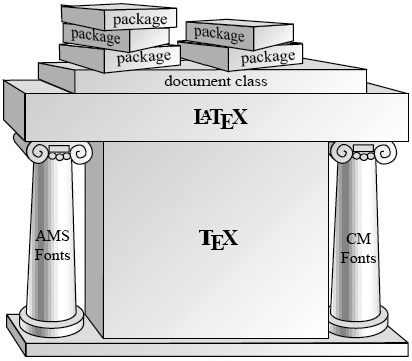
\includegraphics[width=0.65\textwidth]{latexframe}\\
      
\includegraphics[width=0.55\textwidth]{titlepage}\\%scale=0.05
      贴心\alert{秘书}
    %\end{center}
    \end{columns}    
\end{frame}

\begin{frame}{为什么要用\LaTeX?}{Office的那点事}%
  \centering
  
\includegraphics[height=.65\textheight]{msoffice2013.png}\\[.5em]
  \msoffice{} \footnote[frame,1]{及其类似软件(LibreOffice, etc.)}%为了在
                                %beamer中显示脚注,需要使用参数[frame]
  功能异常强大\ldots
\end{frame}

\begin{frame}{为什么要用\LaTeX?}{与Word比较}
  \begin{itemize}
  \item 使用难度
  \end{itemize}
  \centering
  \vspace{2ex}
  \begin{tikzpicture}[scale=0.9, every node/.style={scale=0.9}]
    \pgfplotsset{every axis/.append style={line width=1pt}}
    \begin{axis}[%
      axis x line=bottom,
      axis y line=left,
      ymin=0,
      xtick={},
      xticklabels={},
      xlabel near ticks,
      ytick={},
      yticklabels={},
      ylabel near ticks,
      xlabel={文档大小和复杂性\footnote[frame]{\href{http://www.pinteric.com/miktex.html}{Marko
      Pinteric: http://www.pinteric.com/miktex.html}}},
      ylabel={耗时和难度},
      ]
      \begin{scope}[decoration={random steps,segment length=1pt,amplitude=0.1pt},decorate]
        \addplot [msofficecolour, samples=130, domain=0:2] {1+2*x^3}
                  node[near end, sloped, above] {\msoffice}
                  node[anchor=east, pos=.98] {\tiny (我不玩了!再见\ldots)};
         \addplot [latexcolour, samples=130, domain=0:2] {2+x}
                  node[near end, sloped, above] {\latex};
      \end{scope}
    \end{axis}
  \end{tikzpicture}
\end{frame}

\begin{frame}{为什么要用\LaTeX?}{与Word比较}
  \begin{itemize}
  \item 学习曲线
  \end{itemize}
  \centering
  \vspace{2ex}
  \begin{tikzpicture}[scale=0.9, every node/.style={scale=0.9}]
    \pgfplotsset{every axis/.append style={line width=1pt}}
    \begin{axis}[%
      axis x line=bottom,
      axis y line=left,      
      xtick={},
      xticklabels={},
      xlabel near ticks,
      ytick={},
      yticklabels={},
      ylabel near ticks,
      xlabel={需求复杂度/经验},
      ylabel={学习难度},
      xmin=0,
      xmax=4,
      ymin=0,
      ymax=4,
      ]
      % 用贝塞尔曲线(Bézier curve)绘制学习曲线示意图
      \begin{scope}[decoration={random steps,segment length=1pt,amplitude=0.1pt},decorate]
        \draw[color=msofficecolour] (0,0) .. controls (3.8,0.00) and (1.5,3.8)
        .. (3.8,3.8) node[near end, sloped, above] {\msoffice};
        \draw[latexcolour] (0,0) .. controls (0.1,1.8) and (1.8,1.8)
        .. (3.8,1.6) node[xshift = -0.8cm, sloped, above] {\latex};
      \end{scope}
    \end{axis}
  \end{tikzpicture}
\end{frame}

\begin{frame}{为什么要用\LaTeX?}{Word的那点事}
  \stretchon
  \begin{itemize}
  \item \msoffice 是 \wysiwyg
    \begin{itemize}
    \item ``\textsc{What You See Is What You \emph{Get}}''
    \item 格式和结构有时是含蓄的
    \item 貌似易用,但对排版只能进行有限的控制
    \end{itemize}
    %\myrule
  \item \latex 是 \wysiwym
    \begin{itemize}
    \item ``\textsc{What You See Is What You \emph{Mean}}''
    \item 格式与结构清晰
    \item 貌似繁琐,实则是对版面可以进行详细的控制
    \end{itemize}
  \end{itemize}
  \stretchoff
\end{frame}

\begin{frame}{为什么要用\LaTeX?}{Word的那点事}
  \stretchon
  \begin{itemize}
  \item 玻璃瓶和塑料瓶
    \begin{itemize}
    \item \msoffice 是玻璃瓶$\Rightarrow$ \alert{易碎}
    \item \latex 是塑料瓶$\Rightarrow$ \alert{皮实}
    \end{itemize}
  \item 模板
    \begin{itemize}
    \item \msoffice 往往是\alert{规定}$\Rightarrow$ 沦落为低级趣味的\alert{格式刷}
    \item \latex 强制使用模板$\Rightarrow$ 真正实现了\alert{内容与格式的分离}
    \end{itemize}
  \item 轮子的故事
    \begin{itemize}
    \item \msoffice$\Rightarrow$ \alert{ 发明和制造}轮子
    \item \latex$\Rightarrow$  \alert{ 使用}轮子
    \end{itemize}
  \item 两条腿走路
    \begin{itemize}      
    \item 不会用
      \begin{itemize}
      \item \msoffice $\Rightarrow$ 文档难看,格式丑
      \item \latex $\Rightarrow$ 无法编译,\alert{没有文档}
      \end{itemize}
    \item 会用
      \begin{itemize}
      \item \msoffice $\Rightarrow$ \alert{难看}的文档
      \item \latex $\Rightarrow$ 漂亮的文档
      \end{itemize}
    \item 用的好
      \begin{itemize}
      \item \msoffice $\Rightarrow$ \alert{完美}的文档
      \item \latex $\Rightarrow$ \alert{完美}的文档
      \end{itemize}
    \end{itemize}    
  \end{itemize}
  \stretchoff
\end{frame}

\begin{frame}[fragile]{为什么要用\LaTeX?}{简洁输入优美公式}
  \begin{itemize}
  \item 数学公式\\
    \centering    
    \begin{minipage}{1.0\linewidth}
        \begin{texcode}
                    $$\sum_{p\rm\;prime}f(p) = \int_{t>1}f(t)d\pi(t).$$
                \end{texcode}
    \end{minipage}\\
    \begin{minipage}[h]{0.95\linewidth}
      $$\sum_{p\rm\;prime}f(p) = \int_{t>1}f(t)d\pi(t).$$
    \end{minipage}\\
    \begin{minipage}[h]{1.\linewidth}
      \begin{texcode}
                $$2\uparrow\uparrow k
                \mathrel{\mathop=^{\rm def}}
                2^{2^{\cdot^{\cdot^{\cdot^2}}}}
                \vbox{\hbox{$\Big\}\scriptstyle k$}\kern0pt}.$$
            \end{texcode}
    \end{minipage}\\%[1.3em]
    \begin{minipage}[h]{0.95\linewidth}
      $$2\uparrow\uparrow k
      \mathrel{\mathop=^{\rm def}} 2^{2^{\cdot^{\cdot^{\cdot^2}}}}
      \vbox{\hbox{$\Big\}\scriptstyle k$}\kern0pt}.$$
    \end{minipage}
  \end{itemize}
\end{frame}

\begin{frame}[t,fragile]{为什么要用\LaTeX?}{优雅地绘图}
  \begin{tabular}{cc}
      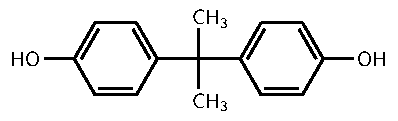
\includegraphics[width=.45\textwidth]{tikzexample/chem.pdf}
    &
      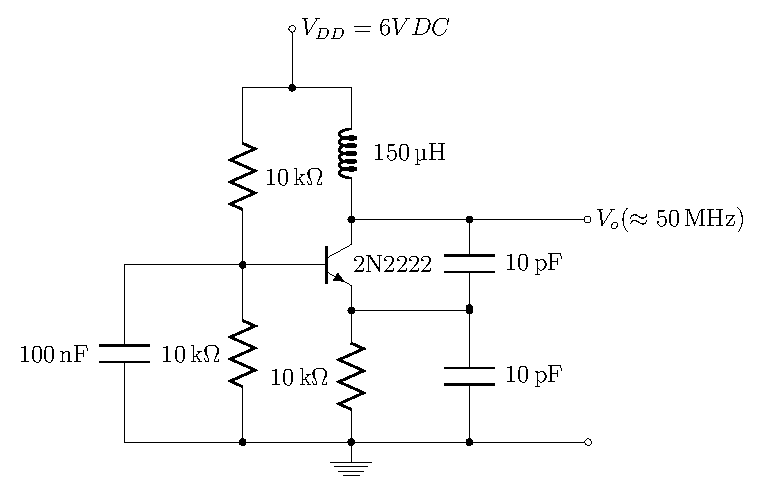
\includegraphics[width=.45\textwidth]{tikzexample/circuitikz.pdf}\\
    
      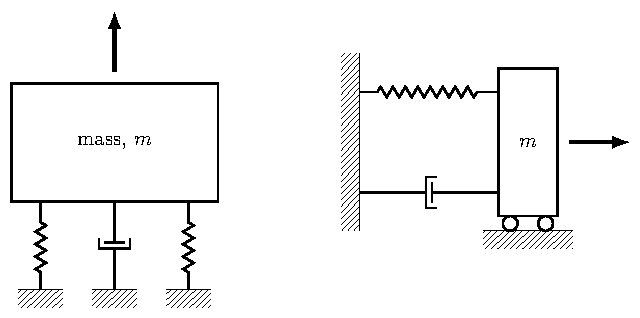
\includegraphics[width=.45\textwidth]{tikzexample/mechanicalsys.pdf}
    &
      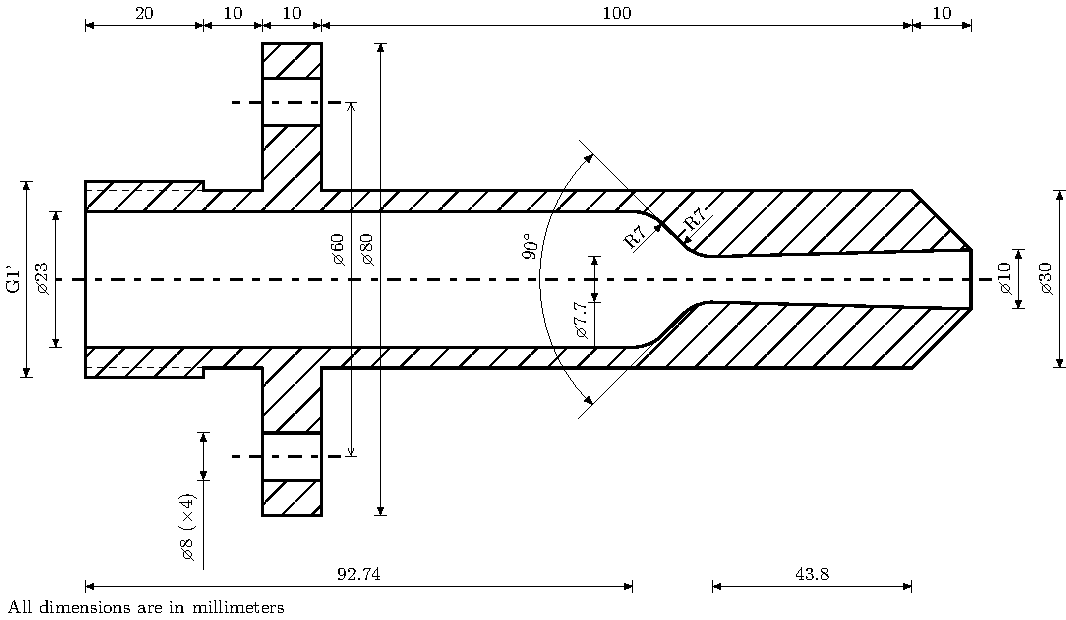
\includegraphics[width=.45\textwidth]{tikzexample/tecdraw.pdf}
  \end{tabular}
\end{frame}

\subsection[是什么?]{什么是\LaTeX ?}\label{sec01-02}
\begin{frame}[t]{什么是\LaTeX?}{排版准备系统}
  \stretchon
  \begin{itemize}
  \item \LaTeX{}是一个功能强大的排版准备系统
  \item \LaTeX{}是标记型语言系统
  %\item \wysiwym
  \item 基于\TeX
    \begin{itemize}
    \item \TeX{}系统提供了300多条基本的排版命令
    \item 允许用户自定义新命令
    \end{itemize}
  \item 有大量的适合特定领域排版需要的的宏包(\url{www.ctan.org},
    \alert{5683}个,\today )
  \end{itemize}
  \stretchoff
\end{frame}

\begin{frame}[t]{什么是\LaTeX?}{工作流程}
  %\stretchon
  \begin{itemize}
  \item \wysiwym\\[4ex]
    %\begingroup
    %\centering
    \begin{center}
      \begin{tikzpicture}[shorten >=1pt,node distance=3cm,auto]
        \draw[%
        -open triangle 60,%
        very thick, ] (0,0) node[anchor=east] (tex)
        {
\includegraphics[height=.2\textheight]{tex_file.png}} --
        (3,0) node[anchor=west] (pdf)
        {
\includegraphics[height=.2\textheight]{pdf_file.png}};
      \end{tikzpicture}
    %\endgroup
    \end{center}
    \vspace{4ex}
  \item \wysiwyg\\[4ex]
    \begin{center}
      
\includegraphics[height=.2\textheight]{word_file.jpg}
    \end{center}
  \end{itemize}
  %\stretchoff
\end{frame}

\begin{frame}[t, fragile]{什么是\LaTeX?}{工作流程}
  \begin{itemize}
  \item 排版流程
  \end{itemize}
  \centering
  \tikzset{ box/.style = {rectangle, draw=black, fill=lightgray} }
  \begin{tikzpicture}
    \node[box] (tex) at(0,0) {.tex};
    \node[box] (pdf) at(8,0) {.pdf};
    \node[box] (dvi) at(0,-4) {.dvi};
    \node[box] (ps) at(8,-4) {.ps};
    \draw[->,very thick, red] (tex) -- node[above]{\alert{\XeLaTeX}} (pdf);
    \draw[->,very thick, red] (tex) -- node[below]{pdf\LaTeX} (pdf);
    \draw[->] (tex) -- node[right]{\LaTeX} (dvi);
    \draw[->] (dvi) -- node[above]{dvips} (ps);
    \draw[->] (ps) -- node[right]{ps2pdf} (pdf);
    \draw[->] (dvi) -- node[above,sloped]{dvipdfmx} (pdf);
  \end{tikzpicture}
  \begin{center}
    \begin{minipage}{0.8\linewidth}
      \footnotesize
      \begin{block}{编译方案}
        \centering
        一般用{pdf\LaTeX}或者{\XeLaTeX}程序直接生
        成\verb|pdf|文件。\\
        如果是\alert{中文}tex文档,\alert{优先}使用\alert{{\XeLaTeX}}程序编译。
      \end{block}
    \end{minipage}
  \end{center}  
\end{frame}

\begin{frame}[t]{什么是\LaTeX?}{特点}
  \stretchon
  \begin{itemize}
  \item 自动编号:一切需要皆有可能
  \item 自动生成目录、索引
  \item 交叉引用:公式、定理、文献、插图、页码等等
  \item PDF输出
  \item 参考文献库
  \item 扩展宏包
  \item \ldots\ldots
  \end{itemize}
  \stretchoff
\end{frame}

\begin{frame}[t, fragile]{什么是\LaTeX?}{自动化处理}
  \stretchon
  \begin{itemize}
  \item 生成目录---\alert{两次}编译\\[3ex]
  %\end{itemize}
  \scalebox{0.8}{ \centering
    \tikzset{box/.style={rectangle, draw=black, fill=lightgray}} 
    \begin{tikzpicture}
      \node (begin) {};
      \node[box] (tex) [right=1 of begin] {.tex源文档};
      \node[box] (latex) [right=1 of tex] {{\LaTeX}引擎};
      \node[box] (pdfdvi)  [right=1  of latex] {PDF/DVI文件};
      \node (end)  [right=1  of pdfdvi] {};
      \node[box] (toc) [above=1.5 of latex] {.toc目录文件};
      \draw[->] (begin) -- node[above]{编写} (tex);
      \draw[->] (tex) -- node[above]{输入} (latex);
      \draw[->] (latex) -- node[above]{输出} (pdfdvi);
      \draw[->] (pdfdvi) -- node[above]{发布} (end);
      \draw[->,dashed,transform canvas={xshift = -0.3cm}] (latex) -- node[left]{前一次编译} (toc);
      \draw[->,dashed,transform canvas={xshift = 0.3cm}] (toc)-- node[right]{再一次编译} (latex);
    \end{tikzpicture}
  }
  %\begin{itemize}
  \item 交叉引用---\alert{两次}编译\\[3ex]
  %\end{itemize}
  \scalebox{0.8}{ \centering
    \tikzset{box/.style={rectangle, draw=black, fill=lightgray}} 
    \begin{tikzpicture}
      \node (begin) {};
      \node[box] (tex) [right=1 of begin] {.tex源文档};
      \node[box] (latex) [right=1 of tex] {{\LaTeX}引擎};
      \node[box] (pdfdvi)  [right=1  of latex] {PDF/DVI文件};
      \node (end)  [right=1  of pdfdvi] {};
      \node[box] (toc) [above=1.5 of latex] {.aux辅助文件};
      \draw[->] (begin) -- node[above]{编写} (tex);
      \draw[->] (tex) -- node[above]{输入} (latex);
      \draw[->] (latex) -- node[above]{输出} (pdfdvi);
      \draw[->] (pdfdvi) -- node[above]{发布} (end);
      \draw[->,dashed,transform canvas={xshift = -0.3cm}] (latex) -- node[left]{前一次编译} (toc);
      \draw[->,dashed,transform canvas={xshift = 0.3cm}] (toc)-- node[right]{再一次编译} (latex);
    \end{tikzpicture}
  }
  \end{itemize}
  \stretchoff
\end{frame}

\begin{frame}[t, fragile]{什么是\LaTeX?}{自动化处理}
  \begin{spacing}{1.0}
    \begin{itemize}
      %\scriptsize
    \item 参考文献---\alert{四次}编译
      \begin{enumerate}
        \scriptsize
      \item 编译.tex源文件生成引用信息、数据库、格式信息.aux辅助文件
      \item 使用biber程序处理第一次编译结果.aux辅助文件,从文献数据
        库提取文献列表代码,生成.bbl文件
      \item 再次编译.tex源文件,处理引用信息,再次生成.aux辅助文件
      \item 第三次编译.tex源文件,生成文献列表
      \end{enumerate}
    \end{itemize}
    \begin{center}
        \scalebox{0.6}{ \centering
        \tikzset{box/.style={rectangle, draw=black, fill=lightgray}} 
        \begin{tikzpicture}
          \node (begin) {编写};
          \node[box] (tex) [right=1 of begin] {.tex源文档};
          \node[box] (xelatex2) [right=1 of tex] {{\XeLaTeX}};
          \node[box] (nocitepdf)  [right=1  of xelatex2] {无引用PDF};
          \node[box] (aux2)  [below=1  of xelatex2] {.aux辅助};
          \node[box] (xelatex3)  [below=1  of aux2] {\XeLaTeX};
          \node[box] (finalpdf)  [right=1  of xelatex3] {最终PDF};
          \node (end)  [right=1  of finalpdf] {发布};
          \node[box] (aux1) [above=1 of xelatex2] {.aux辅助};
          \node[box] (xelatex1) [above=2 of aux1] {\XeLaTeX};
          \node[box] (nobibpdf) [right=1 of xelatex1] {无文献PDF};
          \node[box] (bibtex) [right=2 of aux1] {biber};
          \node[box] (bbl) [right=1 of bibtex] {.bbl文献列表};
          \node (bibtexabove) [above=1 of bibtex] {};
          \node[box] (bib) [left=0.5 of bibtexabove] {\alert{.bib数据库}};
          \node[box] (bst) [right=0.5 of bibtexabove] {.bbx/.cbx\alert{样式文件}};
          \draw[->] (begin) -- (tex);
          \draw[->] (tex) -- node[below]{3} (xelatex2);
          \draw[->] (tex) edge [bend left] node[right]{1} (xelatex1);
          \draw[->] (tex) edge [bend right] node[right]{4} (xelatex3);
          \draw[->] (xelatex2) -- node[below]{3} (nocitepdf);
          \draw[->,dashed] (xelatex2) -- node[left]{3} (aux2);
          \draw[->,dashed] (aux2) -- node[left]{4} (xelatex3);
          \draw[->] (xelatex3) -- node[below]{4} (finalpdf);
          \draw[->] (finalpdf) -- node[below]{4} (end);
          \draw[->,dashed] (xelatex1) -- node[left]{1} (aux1);
          \draw[->] (xelatex1) -- node[above]{1} (nobibpdf);
          \draw[->,dashed] (aux1) -- node[left]{3} (xelatex2);
          \draw[->] (aux1) -- node[below]{2} (bibtex);
          \draw[->] (bib) -- node[left]{2} (bibtex);
          \draw[->] (bst) -- node[right]{2} (bibtex);
          \draw[->] (bibtex) -- node[below]{2} (bbl);
          \draw[->,dashed] (bbl) -- node[above]{3} (xelatex2);
          \draw[->,dashed] (bbl) edge [bend left] node[left]{4} (xelatex3);
        \end{tikzpicture}
      }
    \end{center}
  \end{spacing}
\end{frame}

\begin{frame}[t]{什么是\LaTeX?}{优点}
  \stretchon
  \begin{itemize}
  \item {\color{blue}{高质量的输出:}}\LaTeX{}以排版质量为首要目标
  \item {\color{blue}{超常的稳定性:}}\LaTeX{}系统极少崩溃
  \item {\color{blue}{\LaTeX{}是宏命令编程语言:}}
    \begin{itemize}
    \item 用命令实现排版
    \item 重新定义\LaTeX 命令排版
    \end{itemize}
  \item {\color{blue}{\LaTeX{}是纯文本文件:}}占用空间很小
  \item {\color{blue}{良好的通用性和低廉的价格:}}免费
  \item {\color{blue}{超强的技术支持:}}丰富的网络资源
  \end{itemize}
  \stretchoff
\end{frame}

\begin{frame}[t]{什么是\LaTeX?}{优点}
  \vspace{-3ex}
  \begin{columns}%[c]
    \column{0.4\textwidth}
  \begin{spacing}{0.7}
    \begin{itemize}
    \item \alert{多人}
      \begin{itemize}
      \item 明文编辑
        \begin{itemize}
        \item 方便自由
        \end{itemize}
      \item 版本管理
        \begin{itemize}
        \item 安全可靠
        \item 回滚便捷
        \end{itemize}
      \item 模板丰富
        \begin{itemize}
        \item 学位论文
        \item 科研论文
        \end{itemize}
      \end{itemize}
    \item \alert{多文件}
      \begin{itemize}
      \item 分章节协作
      \item 分专题协作
      \item 分模块协作
      \end{itemize}
    \item \alert{软件}
      \begin{itemize}
      \item 图文分离
        \begin{itemize}
        \item 独立编辑
        \end{itemize}
      \item 表文分离
        \begin{itemize}
        \item 数据文件
        \end{itemize}
      \end{itemize}
    \end{itemize}
  \end{spacing}
  \column{0.55\textwidth}
  \begin{center}
    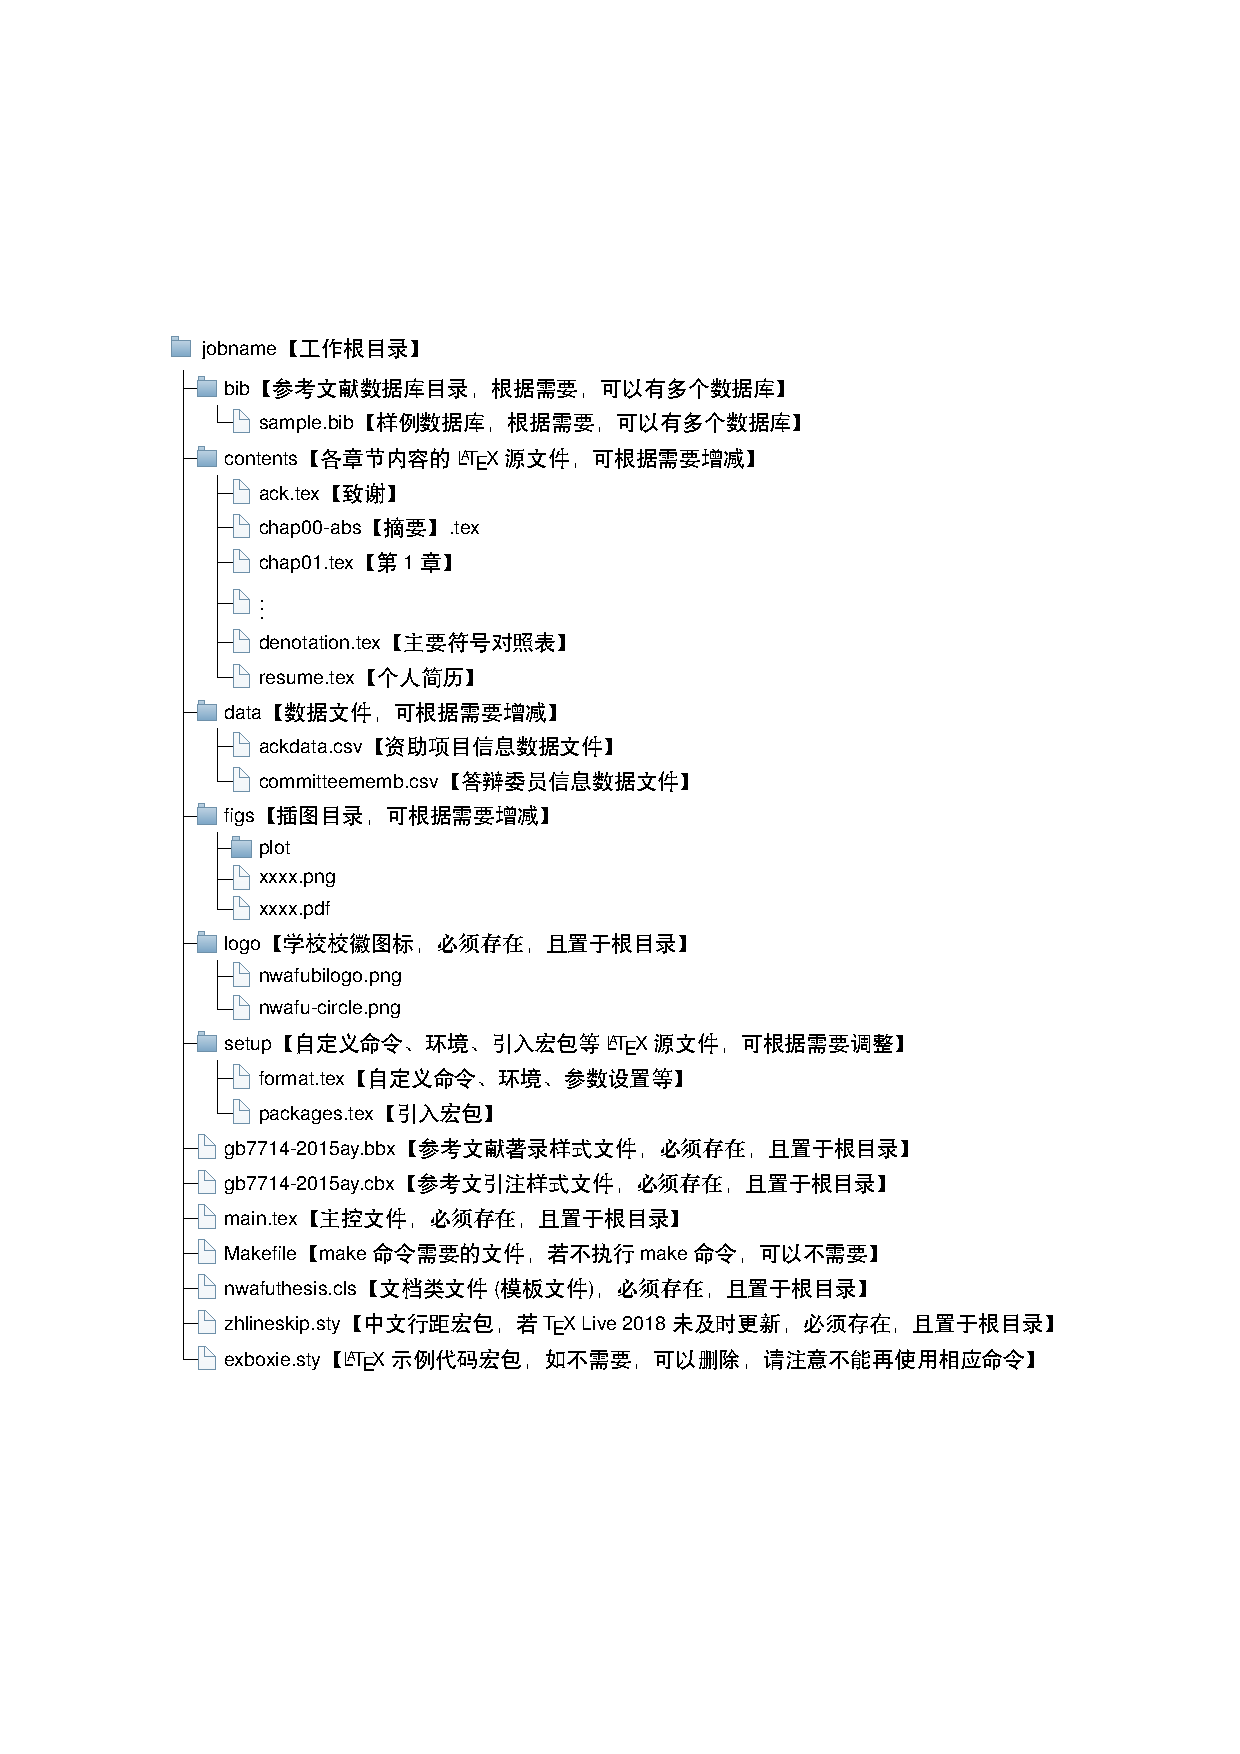
\includegraphics[height=0.72\textheight]{coworks}
  \end{center}
\end{columns}
\end{frame}

\begin{frame}[t]{什么是\LaTeX?}{优点}
  %\stretchon
  \begin{itemize}
  \item 修订管理
    \begin{itemize}
    \item 注释管理
    \item 版本控制
      \begin{itemize}
      \item SVN
      \item Git(回滚、diff)
      \end{itemize}
    \end{itemize}
  \end{itemize}
  \begin{center}
    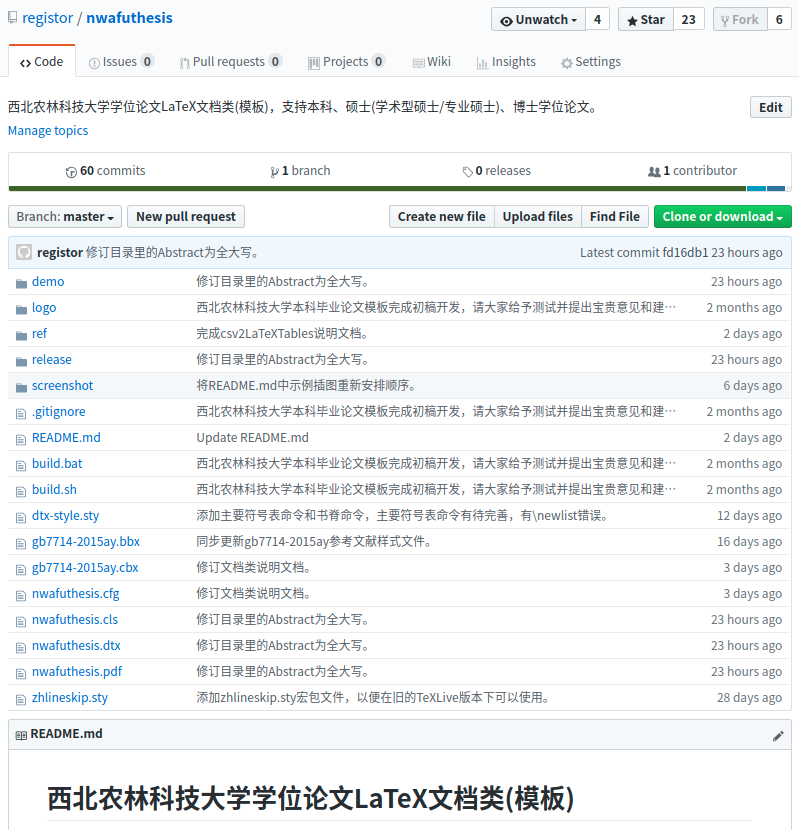
\includegraphics[height=0.5\textheight]{github}\quad
    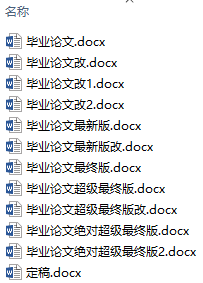
\includegraphics[height=0.5\textheight]{wordver02}\quad
    %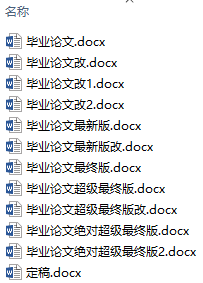
\includegraphics[height=0.4\textheight]{wordver02}
  \end{center}
  %\stretchoff
\end{frame}

\begin{frame}[t]{什么是\LaTeX?}{缺点}
  \stretchon
  \begin{itemize}
  \item 命令繁多
    \begin{itemize}
    \item 常备一本参考资料
    \item 要\alert{多用}
    \end{itemize}
  \item 错误难找:积累经验
  \item 写宏包有难度:普通用户不需要自己写宏包
  \item 使用不直观:目前已有一些所见即所得的扩展
  \end{itemize}
  \stretchoff
\end{frame}

\begin{frame}[t]{什么是\LaTeX?}{PDF文件的批阅批注}
  %\vspace{-3ex}
  % \stretchon
  \begin{columns}[c]
    % \column{0.05\textwidth}
    \column{0.5\textwidth}
    \begin{spacing}{0.9}
    \begin{itemize}%[noitemsep]
    \item \alert{纸质}批注\footnote[frame]{保留\alert{真迹},以作纪念!}
      \begin{itemize}
      \item 打印
      \end{itemize}
    \item
      \alert{平板}批注\footnotemark[\value{footnote}]%\footnotemark[\ref{note
      \begin{itemize}
      %\item GoodNotes
      \item Notability
      \item $\ldots$
      \end{itemize}
    \item \alert{软件}批注
      \begin{itemize}
      \item Adobe Acrobat Pro
      %\item Foxit Reader(福昕)
      %\item Okular
      \item $\ldots$
      \end{itemize}
    \item \alert{源码}批注\footnote[frame]{导师\qtmark{智慧过人、气
          宇不凡、天资聪颖、骨骼精奇},学习\LaTeX 那是\alert{分分钟
          钟}的事!}
      \begin{itemize}
      \item Git版本管理,diff查看
        \begin{itemize}
        \item \href{https://github.com/}{GitHub}
        \item \href{https://gitee.com/}{码云}
        \end{itemize}
      \item 批注宏包
        \begin{itemize}
        \item changes
        %\item todonotes
        \item $\ldots$
        \end{itemize}
      \end{itemize}
    \end{itemize}
    \end{spacing}
  \column{0.45\textwidth}
  \begin{center}
    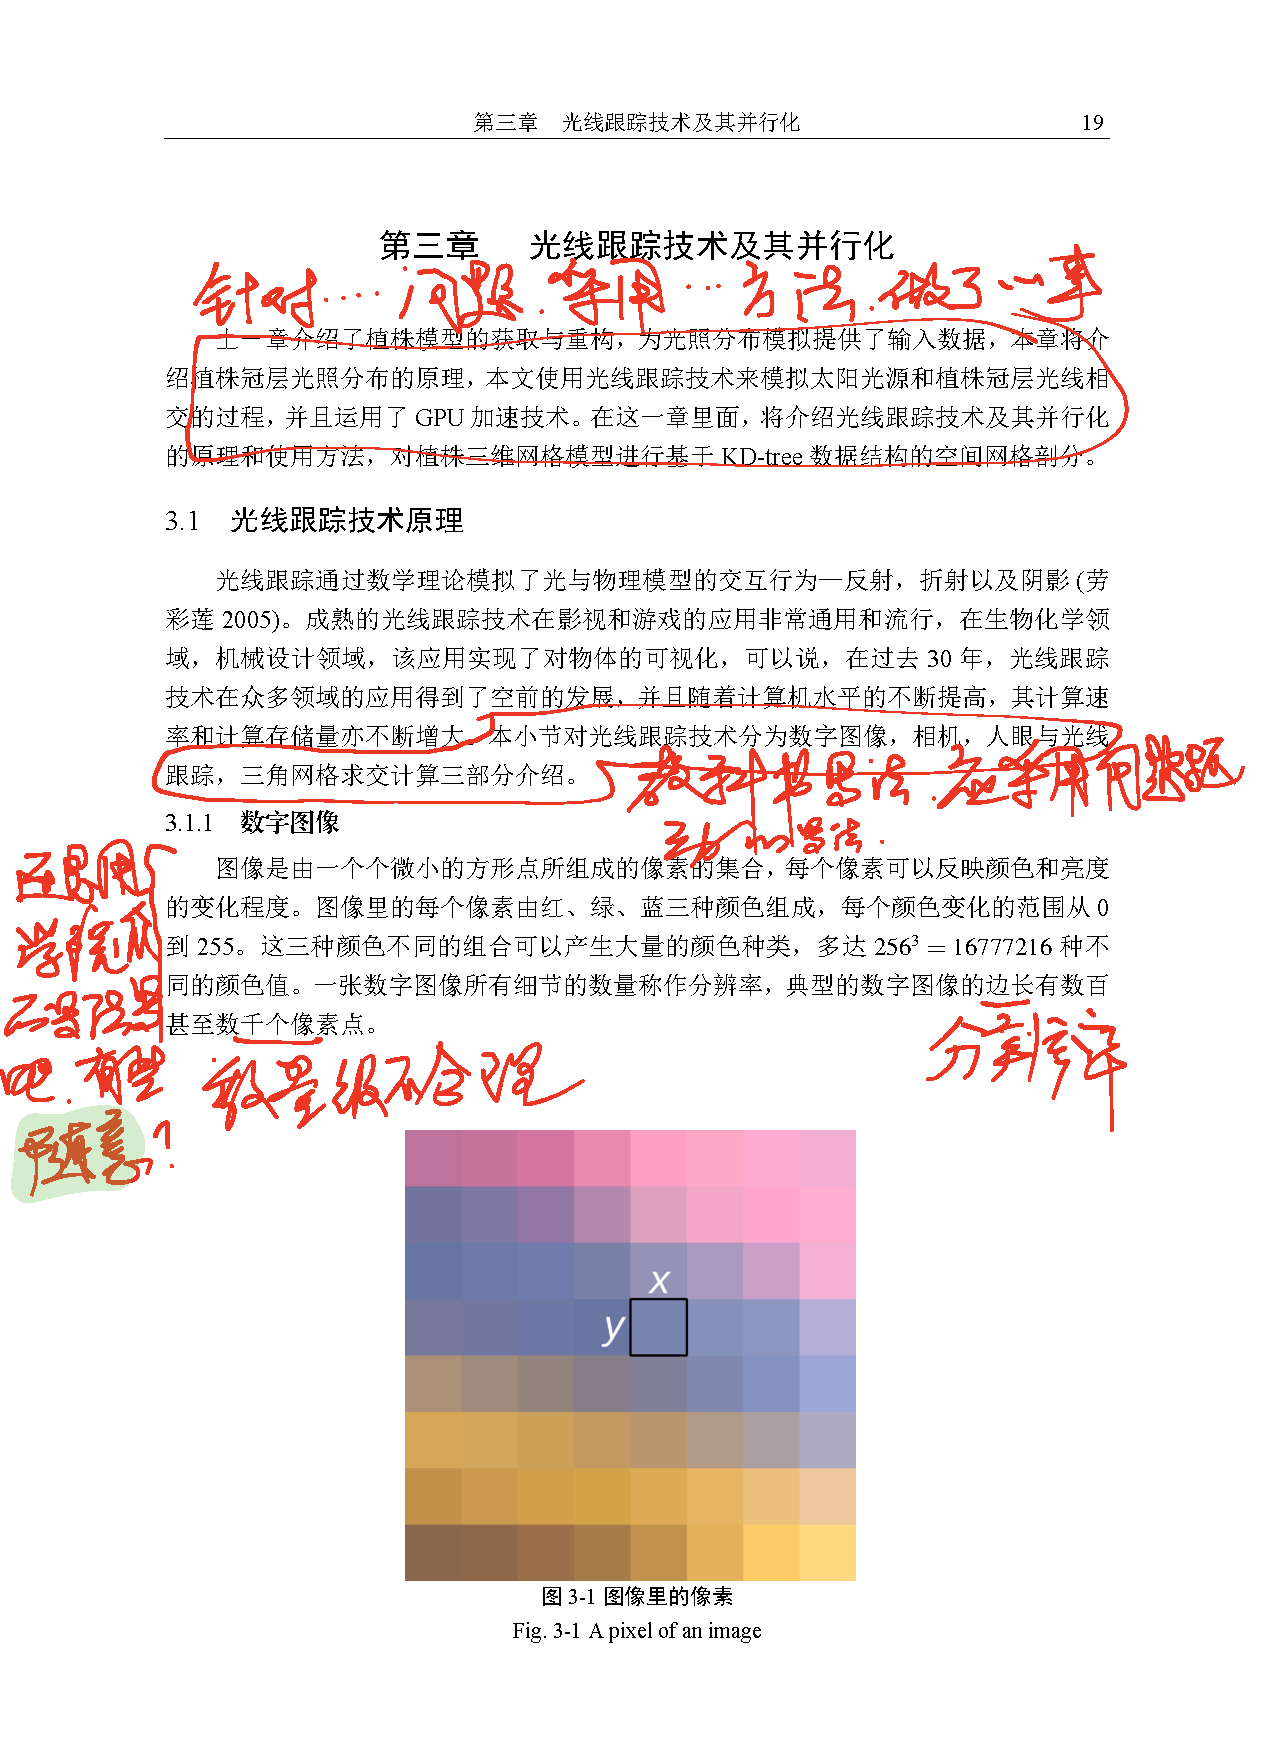
\includegraphics[height=0.35\textheight]{pdftakenotes}\\
    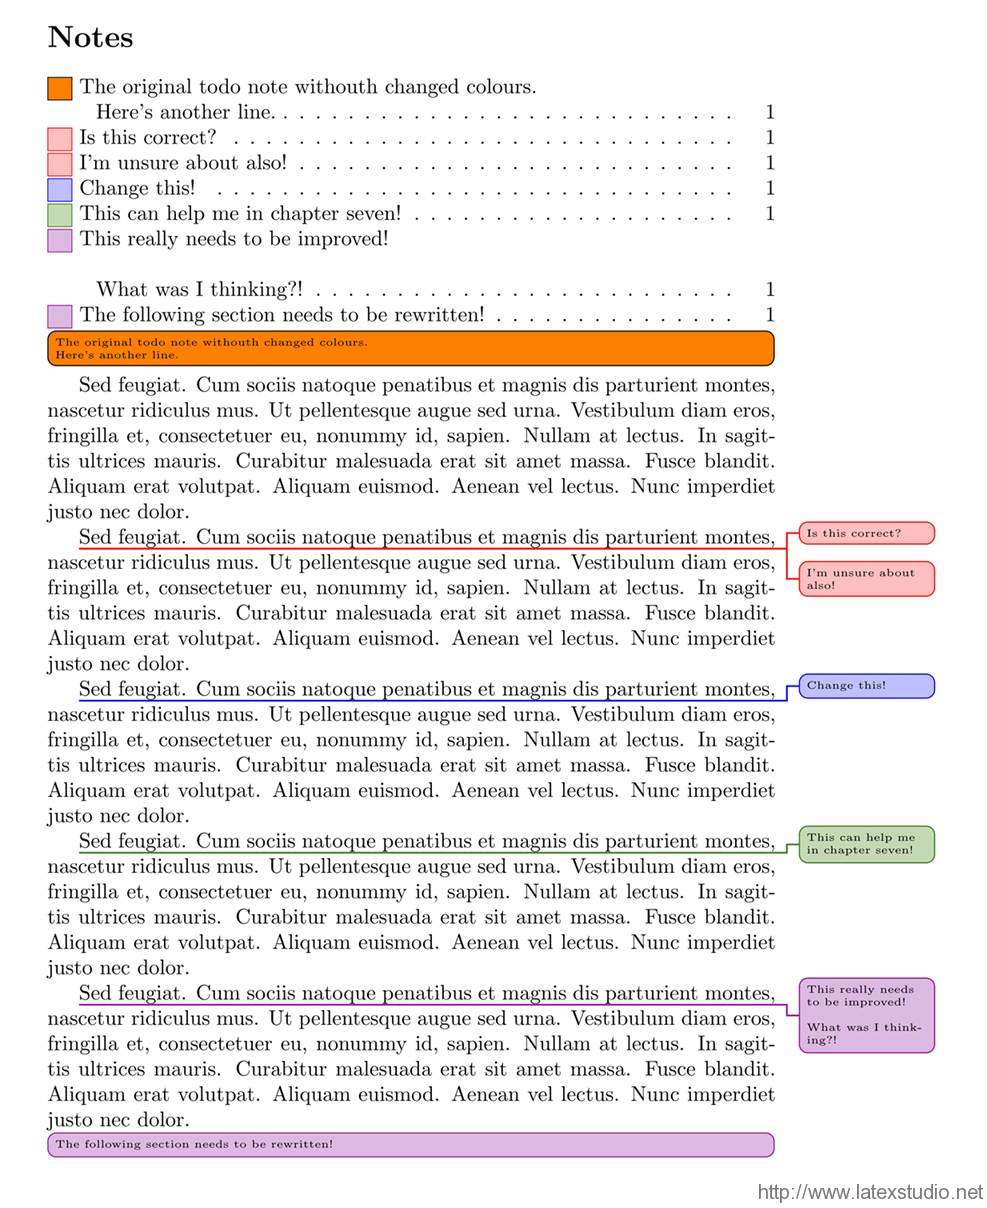
\includegraphics[height=0.35\textheight]{todonotes}
  \end{center}
\end{columns}
% \stretchoff
\end{frame}

\begin{frame}[t]{什么是\latex?}{\latex 的版本}
  \stretchon
  \begin{itemize}
  \item 发行版:
    \begin{itemize}    
    \item Windows:CTex,MikTex,fpTeX
    \item Unix/Linux:teTeX
    \item Mac OS:MacTeX        
    \item 跨平台:\alert{TeXlive},由国际{\TeX}用户组织开发
    \end{itemize}
  \item 编辑器:
    \begin{itemize}
    \item WinEdt,windows平台,收费
    \item \alert{TexStudio},跨平台,免费
    \item Lyx,跨平台,免费
    \item TexMacs,Mac平台,免费
    \item Gummi,Linux平台,免费
    \item Kile,Lunix平台,免费
    \item \ldots\ldots
    \end{itemize}
  \item 在线系统
    \begin{itemize}
    \item
      \href{https://cn.sharelatex.com/}{\alert{ShareLaTeX}: 
        https://cn.sharelatex.com/}%\href{<url>}{<text to display>}.
    \item
      \href{https://www.overleaf.com/}{\alert{Overleaf}: 
        https://www.overleaf.com/}
    \item
      \href{https://v2.overleaf.com/}{\alert{Overleaf V2}: 
        https://v2.overleaf.com/}  
    \end{itemize}
  \end{itemize}
  \stretchoff
\end{frame}

\begin{frame}[t]{什么是\latex?}{处理中文}
  \stretchon
  \begin{itemize}
  \item \alert{\XeTeX}和\alert{\XeLaTeX}
    \begin{itemize}
    \item 底层支持\alert{Unicode}
    \item 字体配置方式灵活
    \item \alert{目前最优的中文处理方式!}
    \item \url{http://scripts.sil.org/xetex}
    \end{itemize}
  \item CCT\alert{外挂}
    \begin{itemize}
    \item 中科院张林波开发
    \item 适合中国国情
    \end{itemize}  
  \item CJK\alert{外挂}
    \begin{itemize}
    \item 德国人 Werner Lemberg 开发
    \item 中文(\alert{C}hinese)、日文(\alert{J}apanese)、韩文(\alert{K}orean)
    \item 缺乏可用的字体
    \item 默认的格式不符合中文排版要求
    \item 不能满足中文的其他要求
    \end{itemize}  
    %\item \url{ftp://ftp.cc.ac.cn/pub/cct/}      
  \end{itemize}
  \stretchoff
\end{frame}

%%%%%%%%%%%%%%%%%%%%%%%%%%%%%% Texlive安装 %%%%%%%%%%%%%%%%%%%%%%%%%%%%%%%%%%%
\section[安装\LaTeX ]{安装\LaTeX 系统}\label{sec01-04}
\subsection[下载]{下载}
\begin{frame}[t]{安装\LaTeX 系统}{下载并启动安装}
  \stretchon
  \emph{以下安装以Windows平台为例}
  \begin{itemize}
  \item 下载并安装\TeX Live
    \begin{itemize}
    \item 在\url{}{https://www.tug.org/texlive/}下载
      \texttt{texlive2018.iso}\footnote[frame]{后续图片不做更
        新,2018与2016的安装过程和注意事项完全相同。}
    \item 将下载到的.iso文件文件刻录到DVD或用虚拟光驱加载
    \item Windows10可以\alert{直接加载}.iso文件
    \item 运行install-tl-advanced.bat批处理文件进行安装
    \end{itemize}
  \end{itemize}
  \vspace{-3ex}
  \begin{columns}[T]
    % \column{0.05\textwidth}
    \column{0.3\textwidth}
  \begin{itemize}  
  \item 其它套件
    \begin{itemize}
    \item \href{http://www.latexstudio.net/page/texsoftware}{\LaTeX 开
        源小屋}
    \end{itemize}
  \end{itemize}
  \column{0.6\textwidth}
  \centering%\vspace{-4ex}
  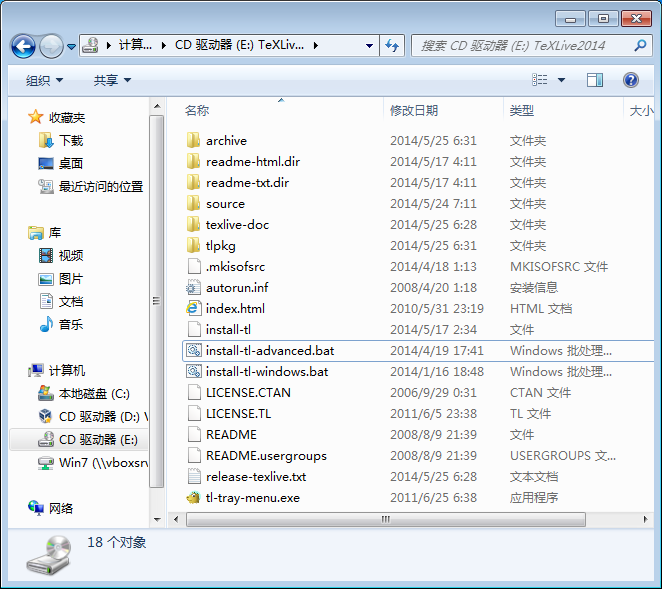
\includegraphics[height=.35\textheight]{texliveinst/fig02-00}
  \end{columns}
  \stretchoff
\end{frame}
\subsection[安装]{安装}
\begin{frame}[t]{安装\LaTeX 系统}{安装选项}
  \begin{itemize}
  \item 启动安装界面
  \item 注意设置\qtmark{修改注册表中的PATH设置}选项为
    \alert{是}\footnote[frame]{否则,需要在安装完成后进行环境变量的手动设置。}
  \end{itemize}
  \centering
  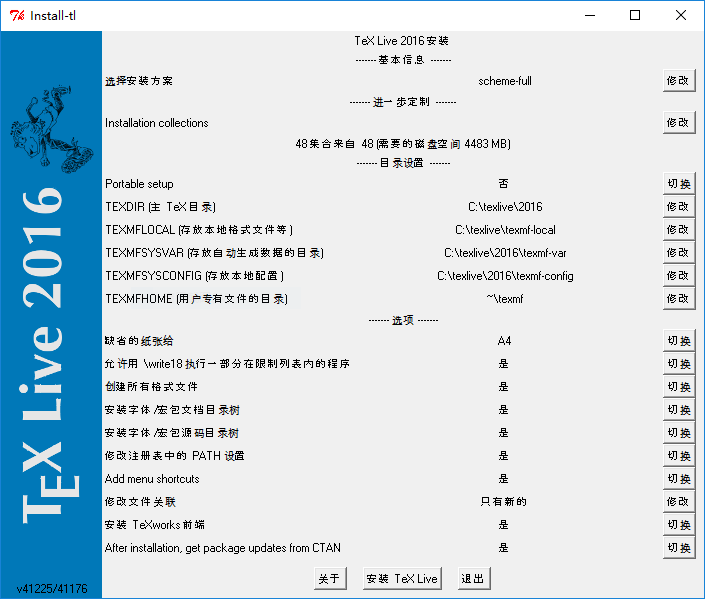
\includegraphics[height=.65\textheight]{texliveinst/fig02-01}
\end{frame}

\begin{frame}[t]{安装\LaTeX 系统}{安装方案}
  \begin{itemize}
  \item 设置安装选项
  \item 可以选择设定的方案
  \end{itemize}
  \centering
  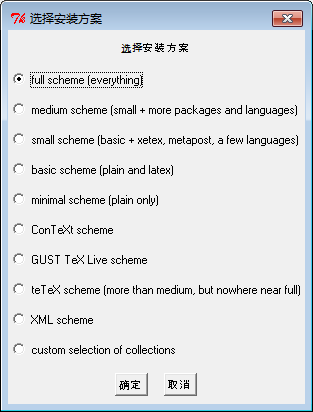
\includegraphics[height=.7\textheight]{texliveinst/fig02-02}
\end{frame}

\begin{frame}[t]{安装\LaTeX 系统}{语言宏包}
  \begin{itemize}
  \item 安装(此处删除了不用的语言宏包,\alert{建议不
      要删除})
  \end{itemize}
  \centering
  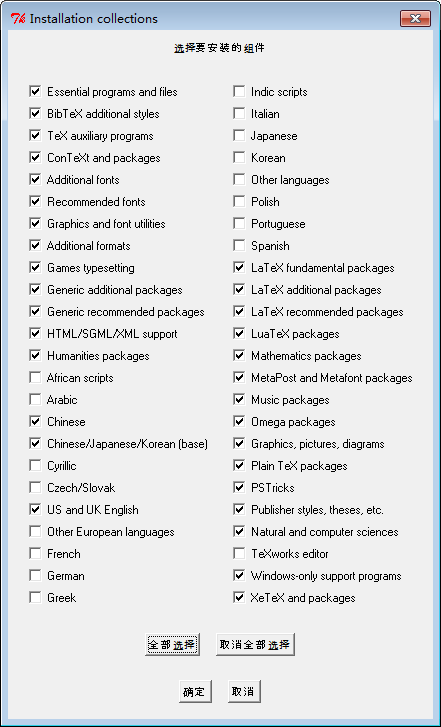
\includegraphics[height=.8\textheight]{texliveinst/fig02-03}
\end{frame}

\begin{frame}[t]{安装\LaTeX 系统}{耐心等待}
  \stretchon
  \begin{itemize}
  \item 耐心等待,直到安装结束
  \end{itemize}
  \centering
  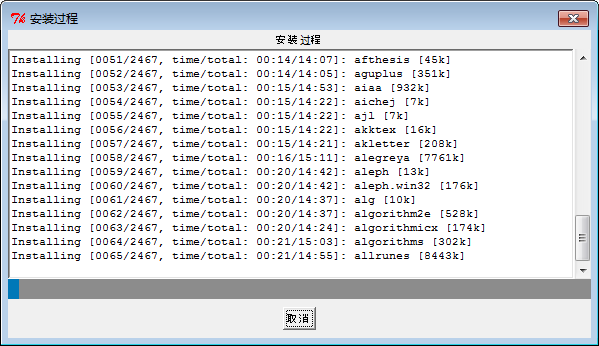
\includegraphics[width=.4\textwidth]{texliveinst/fig02-04} \qquad
  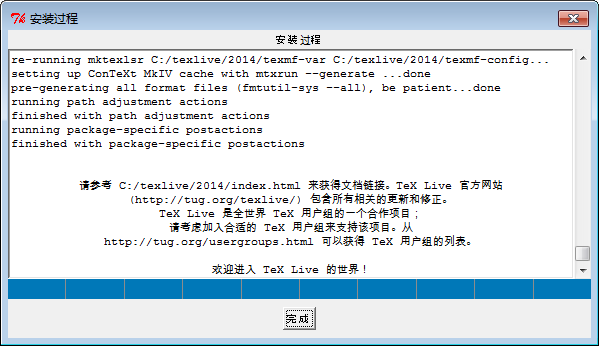
\includegraphics[width=.4\textwidth]{texliveinst/fig02-05}
  \\[4ex]
  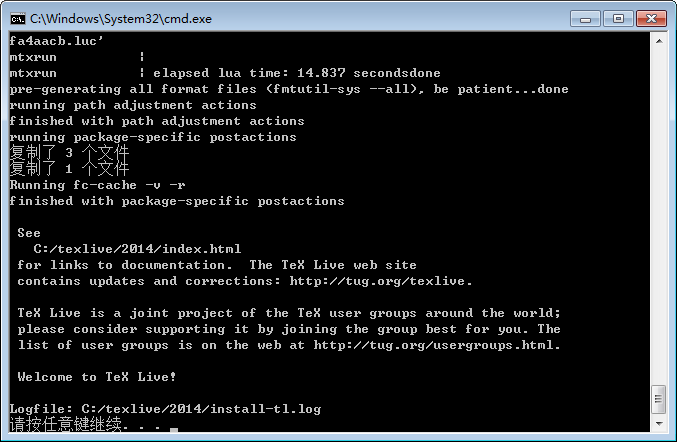
\includegraphics[width=.4\textwidth]{texliveinst/fig02-06}
  \stretchoff
\end{frame}
\subsection[检测]{检测\TeXLive }
\begin{frame}[t]{安装\LaTeX 系统}{检测\TeXLive }
  \stretchon
  \begin{itemize}
  \item 测试,分别在命令行窗口输入:
    \begin{itemize}
    \item {\texttt{tex --version}}
    \item {\texttt{xelatex --version}}
    \end{itemize}
  \end{itemize}
  \centering 
  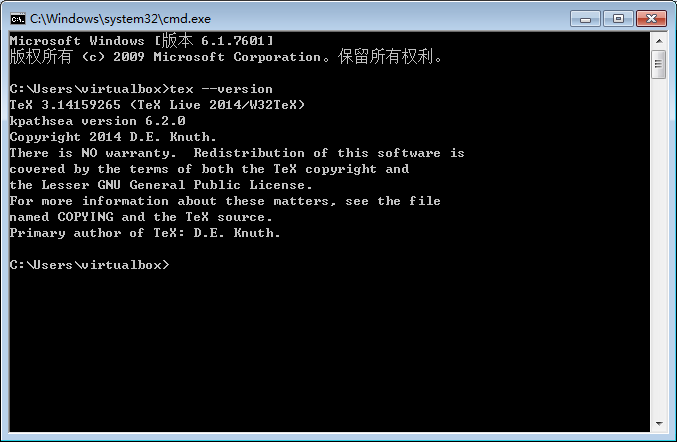
\includegraphics[width=.35\textwidth]{texliveinst/fig02-07}
  \qquad
  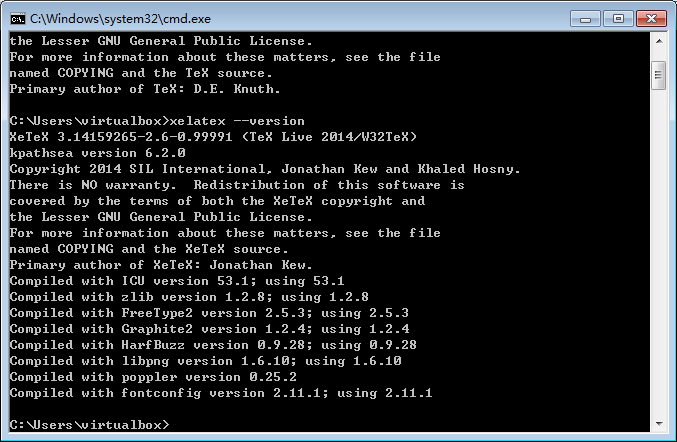
\includegraphics[width=.35\textwidth]{texliveinst/fig02-08}
  \begin{minipage}[h]{0.6\linewidth}
    \begin{block}{测试结果}
      \scriptsize      
      能够正常显示版本号,则表示安装及路径配置成功,若无法正常执行这两
      个命令,请检查PATH路径设置,应该将{\TeX}Live安装路径中
      的\texttt{bin}路径(如:\texttt{C:\textbackslash
        texlive\textbackslash 2018\textbackslash bin\textbackslash
        win32})加入到PATH环境变量中\footnote[frame]{请自行百度
        或Google如何添加环境变量。}。
    \end{block}
  \end{minipage}
  \stretchoff
\end{frame}

\subsection[更新]{更新\TeXLive }
\begin{frame}[t,fragile]{安装\LaTeX 系统}{更新\TeXLive}
  \stretchon
  \begin{itemize}
  \item 设置更新源
    \begin{itemize}
    \item \texttt{tlmgr option repository ctan}或,%
    \item \texttt{tlmgr option repository http://mirror.ctan.org/systems/texlive/tlnet}%  
    % \item {\verb|tlmgr option repository ctan|}或,%
    % \item {\verb|tlmgr option repository http://mirror.ctan.org/systems/texlive/tlnet|}%
    \end{itemize}
  \item 更新{\verb|tlmgr|}程序本身(可选)
    \begin{itemize}
    \item {\verb|tlmgr update --self|}%
    \end{itemize}
  \item 更新\TeXLive 的方法
    \begin{itemize}
    \item 命令行:{\verb|tlmgr update --all|}%
    \item GUI界面:{\verb|tlmgr-gui|}%tlmgr-gui  
    \end{itemize}
    \stretchoff
    \begin{center}
      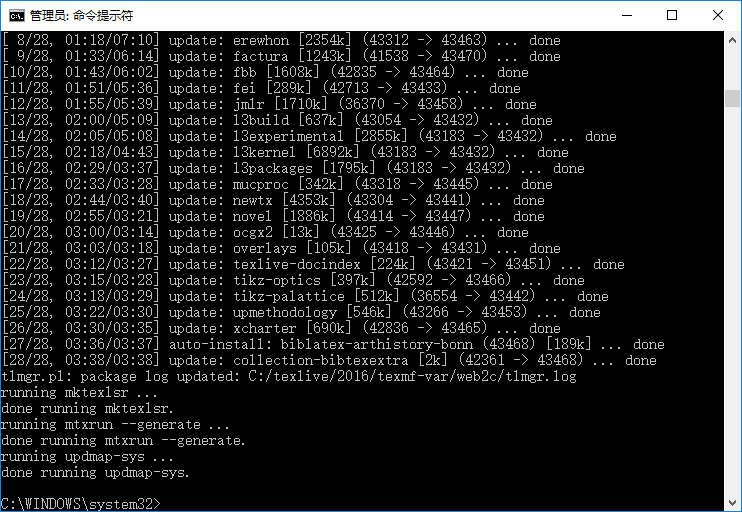
\includegraphics[height=.35\textheight]{texliveinst/updatecmd}\quad
      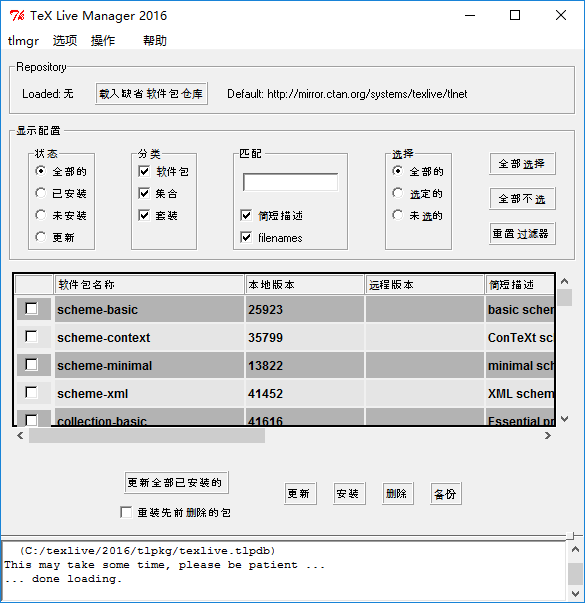
\includegraphics[height=.35\textheight]{texliveinst/updategui}
    \end{center}
  \end{itemize}
\end{frame}

\subsection[测试]{测试\TeXLive }
\begin{frame}{安装\LaTeX 系统}{创建\tex 测试文档}
  \stretchon
  \begin{itemize}
  \item 创建\texttt{testLatex.tex}纯文本文件用于编写{\LaTeX}代码
  \item 创建\texttt{build.bat}批处理文件用于编译{\LaTeX}源文件
  \end{itemize}
  
  \centering%\begin{center}
  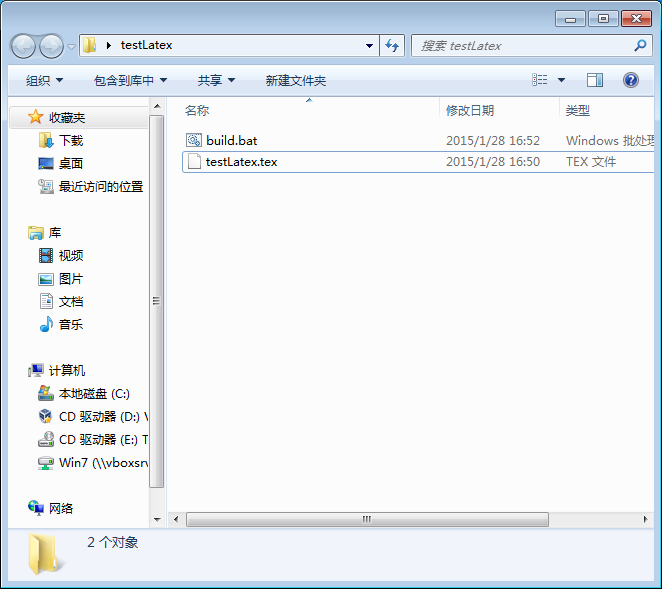
\includegraphics[width=.5\textwidth]{texliveinst/fig02-09}
  % \end{center}
  \stretchoff
\end{frame}

\begin{frame}[t,fragile]{安装\LaTeX 系统}{编写\latex 代码}
  \begin{itemize}
  \item 用记事本打开\verb|testLatex.tex|文件,输入{\LaTeX}代码:
  \end{itemize}
  \centering \vfill
  \begin{minipage}{0.4\linewidth}
    \centering
    \begin{texcode}
           \usepackage{article}

           \begin{document}
              Hell World.
           \end{document}
        \end{texcode}
    
    %\emph{注:后续课程解释}
  \end{minipage}
  \hfill
  \begin{minipage}{0.5\linewidth}
    \centering
    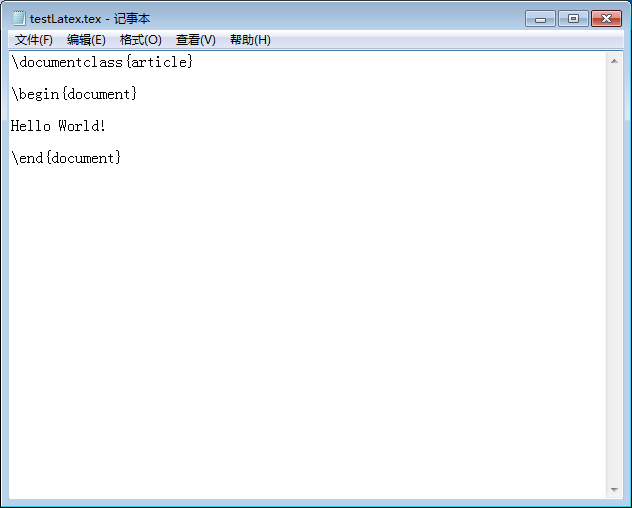
\includegraphics[width=1.0\textwidth]{texliveinst/fig02-10}
  \end{minipage}
\end{frame}

\begin{frame}[t,fragile]{安装\LaTeX 系统}{编写编译批处理文件}
  \begin{itemize}
  \item 用记事本打开\verb|build.bat|文件,输入如下批处理命令:
  \end{itemize}
  \centering \vfill
  \begin{minipage}{0.4\linewidth}
    \centering
    \begin{texcode}
            xelatex testLatex.tex
            del *.log
            del *.aux
        \end{texcode}

    \emph{注:执行编译,\\ 删除中间过程文件}
  \end{minipage}
  \hfill
  \begin{minipage}{0.5\linewidth}
    \centering
    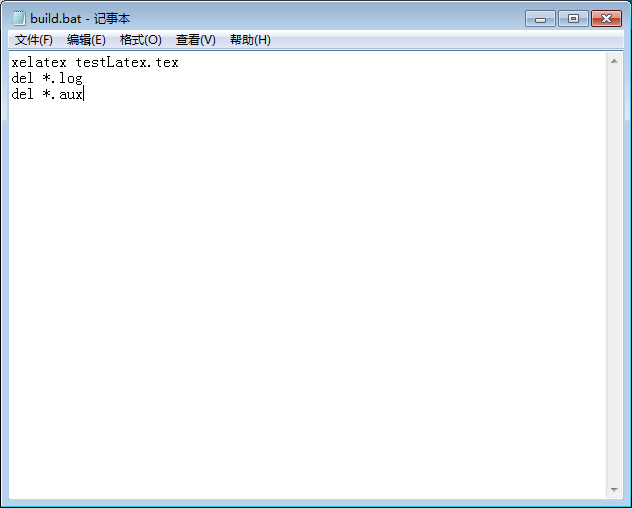
\includegraphics[width=1.0\textwidth]{texliveinst/fig02-11}
  \end{minipage}
\end{frame}

\begin{frame}{安装\LaTeX 系统}{编译\latex 源代码文件}
  \stretchon
  \begin{itemize}
  \item 执行\texttt{build.bat}编译{\LaTeX}源文件\texttt{testLatex.tex}
  \item 得到\texttt{testLatex.pdf}结果文件
  \end{itemize}

  \centering
  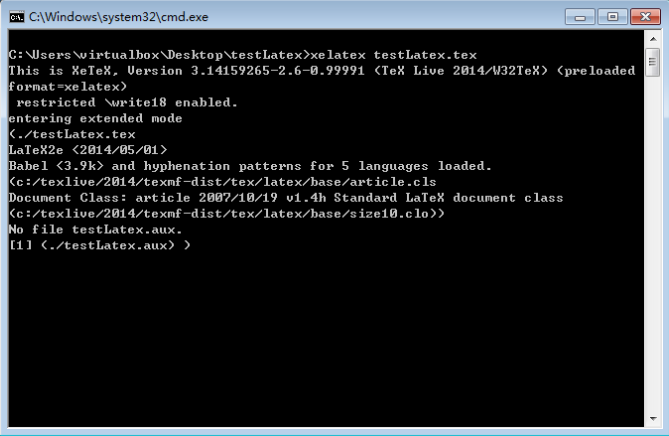
\includegraphics[height=.35\textheight]{texliveinst/fig02-12-2}
  \qquad
  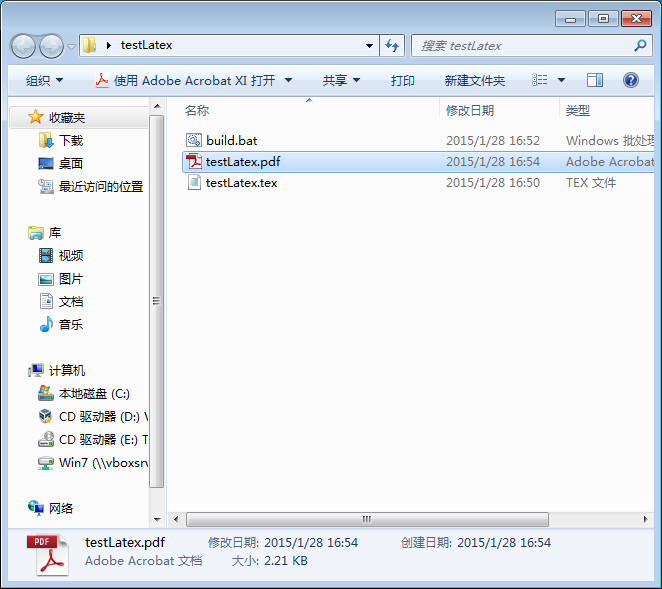
\includegraphics[height=.35\textheight]{texliveinst/fig02-12}
  \stretchoff
\end{frame}

\begin{frame}[t]{安装\LaTeX 系统}{查看编译结果}
  \stretchon
  \begin{itemize}
  \item 双击\texttt{testLatex.pdf}查看生成的到\texttt{pdf}文件
  \end{itemize}
  \centering
  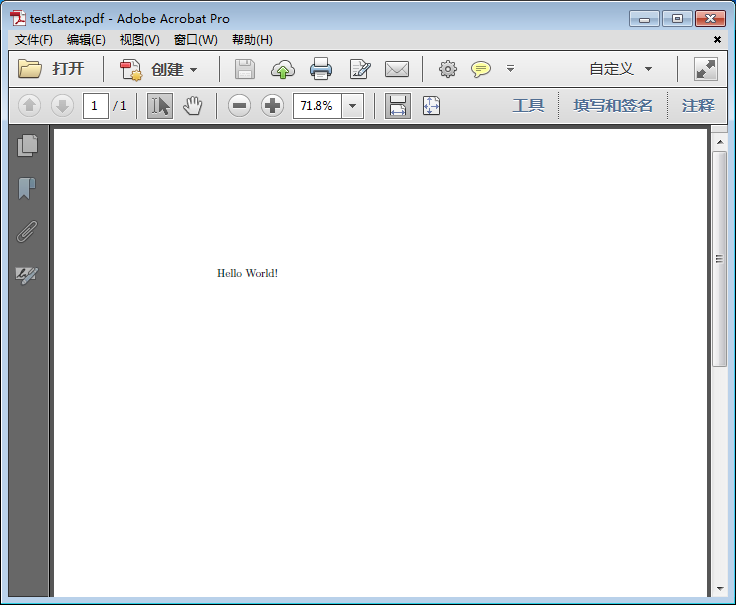
\includegraphics[width=.6\textwidth]{texliveinst/fig02-13}
  \begin{minipage}[h]{0.4\linewidth}
    \begin{block}{结果正确}
      \scriptsize
      \centering
      到此,表示{\TeX}Live安装正常,能够正常工作,配置成功。
    \end{block}
  \end{minipage}
  \stretchoff
\end{frame}

\begin{frame}[t]{安装\LaTeX 系统}{网络安装方式}
  \stretchon
  \begin{itemize}
  \item 通过网络在线安装与上述过程类似,可参
    考\url{http://www.tug.org/texlive/}的指导进行安装
  \item 安装结束后,也可以按上述方式进行测试
  \end{itemize}
  \centering
  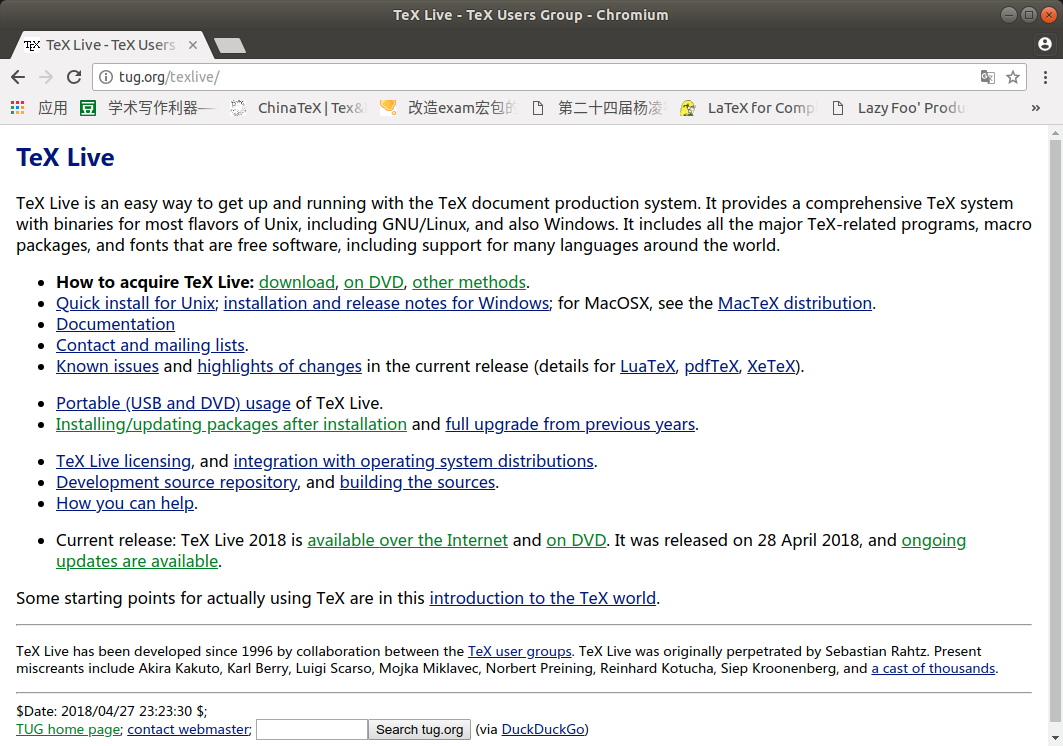
\includegraphics[width=.55\textwidth]{texliveinst/fig02-000}
  \stretchoff
\end{frame}

\subsection[IDE]{IDE环境}
\begin{frame}[t]{安装\LaTeX 系统}{安装编辑器}
  \stretchon
  \begin{itemize}
  \item 可以使用任何一个编辑器做为\LaTeX 的IDE:
  \end{itemize}
  \centering
  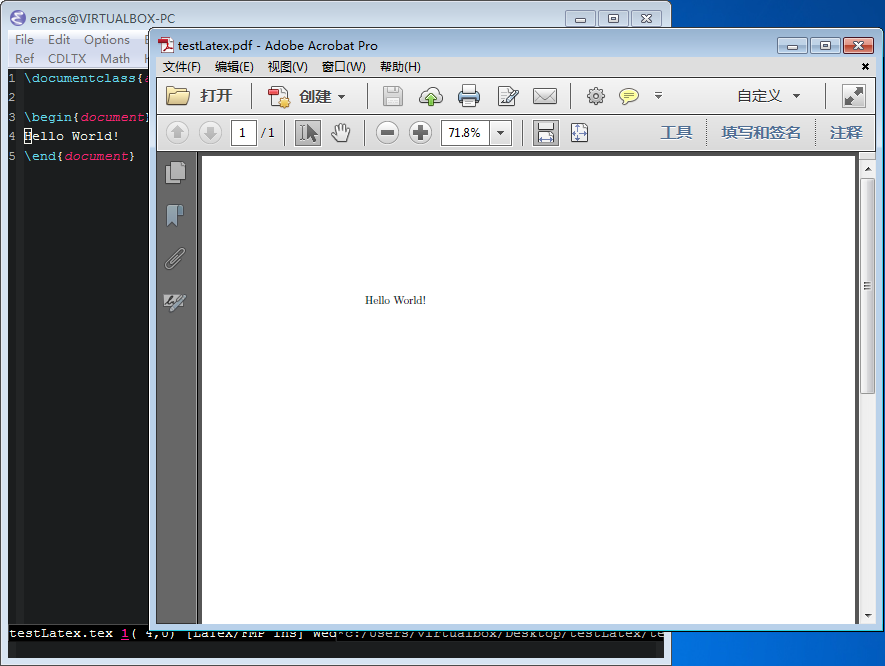
\includegraphics[height=.3\textheight]{texliveinst/fig02-22} \qquad
  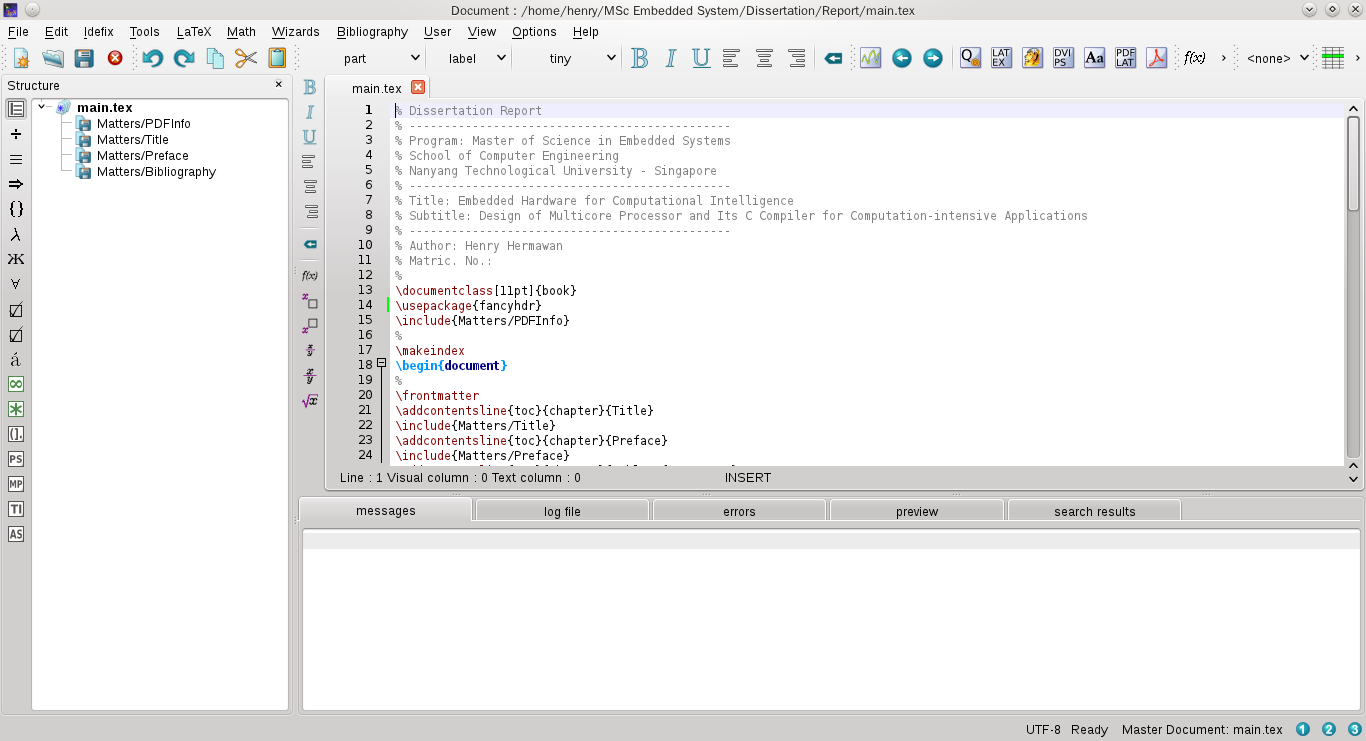
\includegraphics[height=.3\textheight]{texliveinst/texstudio}
  \\[1ex]
  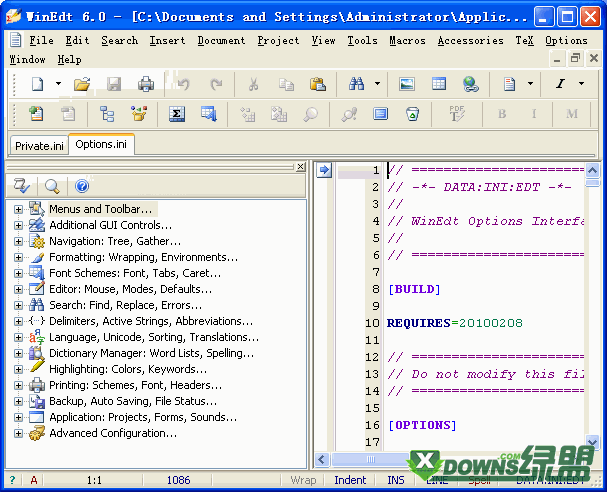
\includegraphics[width=.3\textwidth]{texliveinst/WinEdit}
  \stretchoff
\end{frame}
%%%%%%%%%%%%%%%%

\section[学习\LaTeX ]{学习\LaTeX}\label{sec03}
\subsection{学习资源}
\begin{frame}[t]{学习\LaTeX}{参考资料}
  \stretchon
  \begin{itemize}
  \item \alert{免费}电子文档
    \begin{itemize}
    \item \TeXLive 帮助文档(\TeXLive 中的\alert{\texttt{texdoc}}命令
      )
    \item \url{http://202.117.179.110},耿楠的文档和微视频
    \item 耿楠\qtmark{\LaTeX 排版技术}蓝墨云班课班课号:332948
    \item 一份不太简短的{\LaTeXe}介绍(\texttt{texdoc lshort-zh})
    %\item \LaTeX~排版学习笔记,97页,简单。
    %\item \LaTeX~NOTES V2,213页,简单全面。
      % \item Emacs + {\LaTeX}快速上手,74页,主要讲高效编辑{\LaTeX}代
      %   码。
    \end{itemize}
  \item 纸质教材和专著
    \begin{itemize}
    \item {\LaTeX}~入门-刘海洋,详细全面
    \item {\LaTeXe}~完全学习手册(第2版)-胡伟,详细全面
    \end{itemize}
  \item \texttt{BBS}论坛
    \begin{itemize}
    \item \url{http://www.latexstudio.net/},{\LaTeX}工作室(中文)%
    \item \url{http://www.ctan.org/},最新、稳定的{\LaTeX}老家%
    \end{itemize}
    % \item \url{http://bbs.ctex.org/forum.php},中文论坛。
    % \item \url{http://bbs.chinatex.org/forum.php},中文论坛。
  \end{itemize}
  \stretchoff
\end{frame}

\subsection[文档结构]{\latex 的文档结构}\label{sec02-02}
\begin{frame}[t, fragile]{学习\LaTeX}{文档结构}
  \begin{columns}
    \begin{column}{0.5\textwidth}      
      \begin{itemize}
      \item {\only<2>{\color{red}}引入文档模板命令}\\
        \begin{itemize}
        \item {\only<2>{\color{red}}\textbackslash documentclass}
        \end{itemize}
      \item {\only<3>{\color{red}}导言区} \par
        用于设置全局命令
        \begin{itemize}
        \item {\only<4>{\color{red}}宏包} \par
          扩展基本\latex 命令
        \item {\only<5>{\color{red}} 定义/命令/宏}\par
          用户自定义的命令
        \end{itemize}
      \item {\only<6>{\color{red}}文稿}
        \begin{itemize}
        \item {\only<7>{\color{red}}命令} \par
          影响参数内部文本或是\{...\}区块中文本%
        \item {\only<8>{\color{red}}环境} \par
          只影响环境内部文本
        \end{itemize}
      \end{itemize}
    \end{column}

    \begin{column}{0.45\textwidth}
      \begin{block}{.tex file}
        {
          \tiny \ttfamily
         {\only<2>{\color{red}} \textbackslash documentclass[letterpaper, 11pt]\{article\}} \par
         {\only<3>{\color{red}}\% 导言区 \par          
          \quad {\only<4>{\color{red}} \% 宏包 \par
          \quad \textbackslash usepackage[margin=2.5cm]\{geometry\} \par
          \quad \textbackslash usepackage\{graphicx\} \par
          \quad ...} \par
         \quad {\only<5>{\color{red}} \% 自定义命令 \par
         \quad \textbackslash newcommand\{name\}[num]\{definition\} \par
         \quad ...}
       }\par
         
       \par
       {\only<6>{\color{red}} \% 文稿 \par
       \textbackslash begin\{document\} \par
       ... \par
       \quad {\only<7>{\color{red}}\textbackslash section\{...\}} \par
       \quad ... \par
       \qquad {\only<7>{\color{red}}\textbackslash subsection\{...\}} \par
       \qquad ... \par
       \quad \qquad {\only<8>{\color{red}}\textbackslash
       begin\{equation\} \par
       \quad \qquad ... \par
       \quad \qquad \textbackslash end\{equation\}} \par
       \qquad ... \par
       \quad {\only<7>{\color{red}}\textbackslash section\{...\}} \par
       ... \par
       \par
       \textbackslash end\{document\} \par
       } }
     \end{block}
   \end{column}
 \end{columns}
\end{frame}

\begin{frame}[t, fragile]{学习\LaTeX}{命令和环境}
  \stretchon
  \begin{itemize}
  \item 文稿({\TeX}源文件)
    \begin{itemize}
    \item 正文
    \item 排版控制命令
    \end{itemize}
  \item 排版控制命令:用\alert{倒斜线}引导的字符串
    \begin{itemize}
    \item 控制字:一个或多个字母构成,区分大小写,如:\texinline{\alpha}
    \item 控制符:一个特殊字符构成,如\texinline{\%}
    \end{itemize}
  \item 排版命令的参数:\\
    \fbox{%
      \textbackslash {\color{blue}{排版命令}}[{\color{green}{可选参
          数}}]$\left\{\text{\color{red}{其它参数}}\right\}$ }%
    \begin{itemize}
    \item 方括号中的参数为可选
    \item 花括号中的其它参数是不可省略的参数
    \item 命令也可以不带参数
    \end{itemize}
  \item 环境: \texinline{\begin{xxx}}和\texinline{\end{xxx}}之间的内容
    \begin{itemize}
      \item \alert{一篇文章有且只能有一个\texinline{document}环境}
    \end{itemize}
  \end{itemize}
  \stretchoff
\end{frame}

\begin{frame}[t,fragile]{学习\LaTeX}{中文文档}
  \begin{spacing}{1.3}
    \begin{itemize}
    \item 中文文稿{\latex}文档实例
      \begin{itemize}
      \item 文档类:\texinline{\documentclass{ctexart}}
        \begin{itemize}
        \item \texinline{ctexart}、\texinline{ctexbook}、\texinline{ctexrep}、\texinline{ctexbeamer}等
        \item 12pt表示基本字体大小
        \end{itemize}
      \end{itemize}
    \end{itemize}    
    \begin{center}
    %\hfill
    \begin{minipage}{0.38\linewidth}
      \begin{center}
        \texfile{./code/302.tex}
      \end{center}
    \end{minipage}
    \begin{minipage}{0.3\linewidth}
      
\includegraphics[scale=0.3]{fig03-02}
    \end{minipage}
    \end{center}
  \end{spacing}
\end{frame}

\begin{frame}[t,fragile]{学习\LaTeX}{基本约定}
  \stretchon
  \begin{itemize}
  \item 分组:\{ \ldots\ldots \}
    \begin{itemize}
    \item 欢迎你来到{\latex}(\verb|{\LaTeX}|)世界,
    \end{itemize}
  \item 注释:\%开始的一行
  \item 西文标点后要加空格
  \item 建议各种环境的开始和结束各占一行
  \item 换行:1个回车为1个空格,2个以上回车为1个换行
  \end{itemize}
  \stretchoff
\end{frame}

\subsection{处理错误}
\begin{frame}[t, fragile]{常见错误}{命令未定义}
  \stretchon
  \begin{itemize}
  \item 命令名称\alert{输入}错误\\[3ex]
  
  
  比如将 \texinline{\author{作者}} 错写为 \texinline{\authos{作者}},
  编译后将会看到如下错误信息:
  \begin{texcode}
    ! Undefined control sequence.
    l.12 \authos
  \end{texcode}
  其中第一行说明错误原因是“命令未定义”,第二行说明错误出现在第 12行
  的 \texinline{\authos} 这里。
  \end{itemize}
  \stretchoff
\end{frame}

\begin{frame}[t, fragile]{常见错误}{缺少\$ 、\$\$等符号}
  \stretchon
  \begin{itemize}
  \item 例如缺少\$号\\[3ex]
  
  
  第二常见的错误是忘记将公式放在一对 \texinline{$} 里面.
  比如将 \texinline{$2^3=8$} 错写为 \texinline{2^3=8},
  编译后将会看到如下错误信息:
  \begin{texcode}
    ! Missing $ inserted.
    <inserted text>
                    $
    l.19 2^
           3=8
  \end{texcode}
  其中第一行说明错误原因是“缺少\$号”,后面几行说明错误出现在第 19行
  的 \texinline{2^3=8} 这里。
  \end{itemize}
  \stretchoff
\end{frame}

\begin{frame}[t, fragile]{常见错误}{括号不配对}
  \stretchon
  \begin{itemize}
  \item 例如花括号\}不配对\\[3ex]
  
  
  第三常见的错误是花括号无法配对.
  比如将根号 \texinline!$\sqrt{2}$! 错写为 \texinline!$\sqrt{2]$!,
  编译后将会看到如下错误信息:
  \begin{texcode}
    ! Missing } inserted.
    <inserted text>
                    }
    l.17 $\sqrt{2]$
  \end{texcode}
  其中第一行说明错误原因是“缺少 \} 号”,后面几行说明错误出现在第 17
  行这里。
  \end{itemize}
  \stretchoff  
\end{frame}

\section[\nwafuthesis]{\nwafuthesis 毕业论文模板简介}
\subsection[开发需求]{开发需求}
\begin{frame}[t]{\nwafuthesis 模板}{开发需求}
  \stretchon
  \begin{itemize}
  \item \href{https://yjshy.nwafu.edu.cn/xwgl/xwlwxzgf/index.htm}{研究生学位论文写作指南}
  \item \href{https://jiaowu.nwsuaf.edu.cn/tzgg/34321.htm}{本科生毕业论文(设计)写作规范}
  \end{itemize}
  \centering
  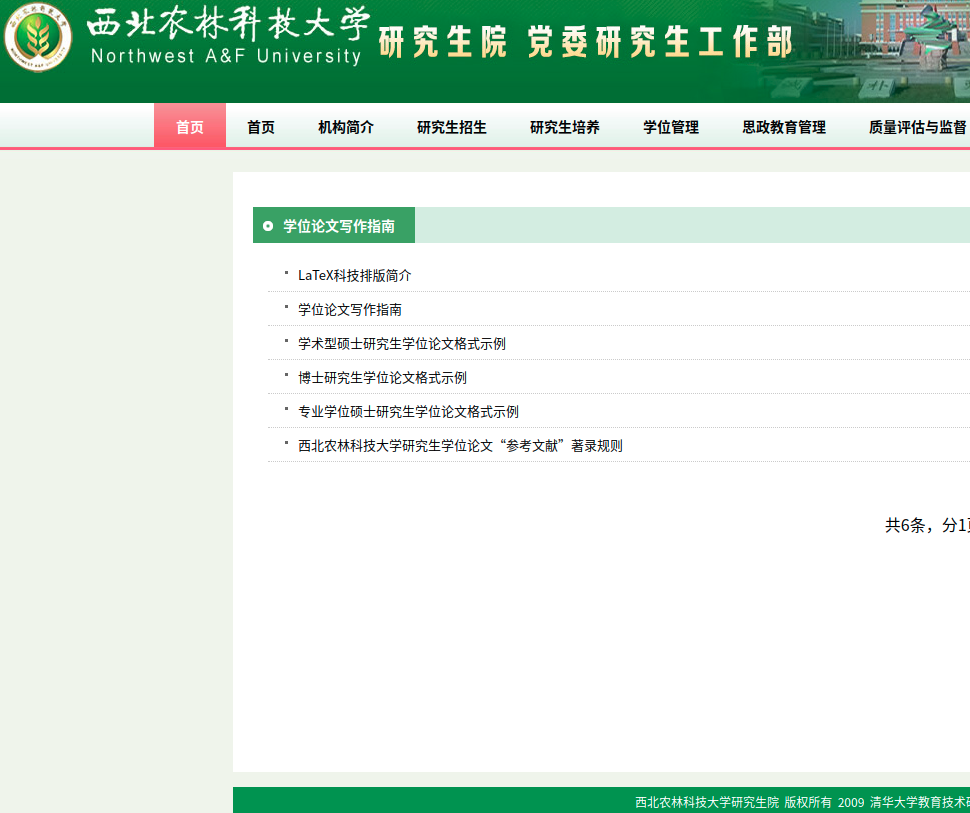
\includegraphics[height=0.4\textheight]{yjshxwb}\quad
  
\includegraphics[height=0.4\textheight]{jiaowuchu}
  \stretchoff
\end{frame}

\subsection[模板下载]{模板下载}
\begin{frame}[t]{\nwafuthesis 模板}{模板下载}
  \stretchon
  \begin{itemize}
  \item \href{https://github.com/registor/nwafuthesis}{GitHub开源托管
      (\alert{推荐})}\footnote[frame]{问题反馈与讲座、实时更新在GitHub
      发布。}
    \begin{itemize}
    \item 模板必须文件
      \begin{itemize}
      \item \LaTeX 文档类(模板): \qtmark{nwafuthesis.cls}
      \item 文献著录样式文件:\qtmark{gb7714-2015ay.bbx}
      \item 文献引注样式文件:\qtmark{gb7714-2015ay.cbx}
      \item 中文行距调整宏包:\qtmark{zhlineskip.sty}
      \item 学校图标:logo文件夹
      \end{itemize}
    \item demo 示例文件夹
    \item release 打包下载
    \end{itemize}
  \item \href{http://202.117.179.110/}{信息学院师生互动平台}
  \item 西农教学发展研讨QQ群
  \end{itemize}
  % \centering
  % 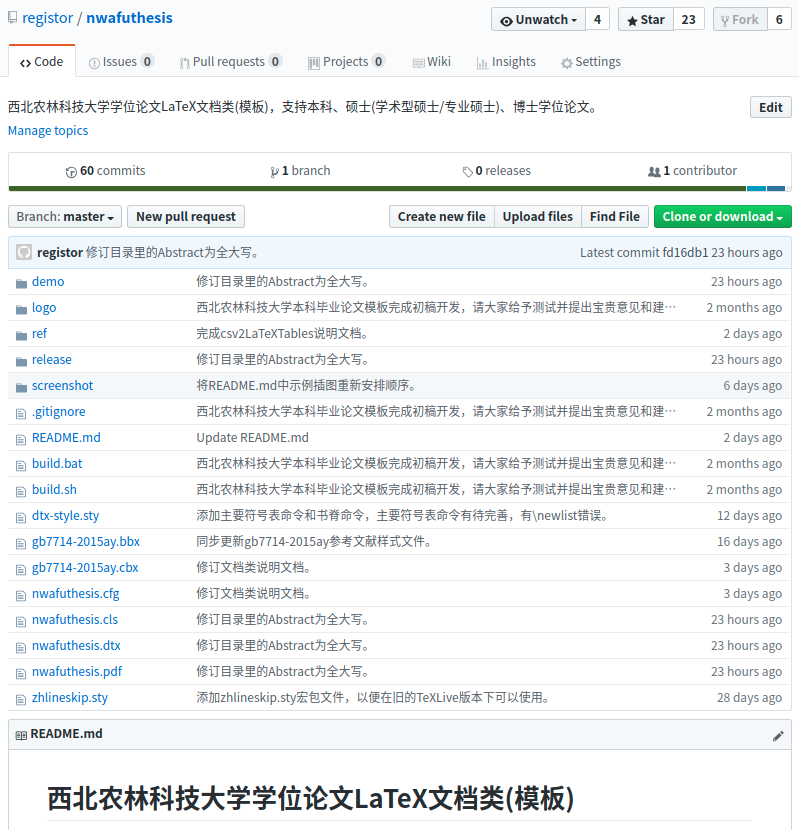
\includegraphics[height=0.6\textheight]{github}
  \stretchoff
\end{frame}

\subsection[模板使用]{模板使用}
\begin{frame}[t]{\nwafuthesis 模板}{模板使用}
  \stretchon
  \begin{itemize}
  \item \href{http://www.latexstudio.net/page/texsoftware}{安装\TeX 套件}
    \begin{itemize}
    \item 跨平台:\TeX Live (\alert{推荐},建议不低于2018版)
    \item Windows:Mi\TeX 
    \item MacOS:Mac\TeX
    \end{itemize}
  \item 安装IDE
    \begin{itemize}
    \item Windows:WinEdt
    \item 跨平台:TexStudio
    %\item 跨平台:Vim/Emacs
    %\item 记事本:notepad++、gedit等
    \item $\ldots$
    \end{itemize}
  \item 用\texinline{\documentclass{nwafuthesis}}引入文档类(模板)
    \begin{itemize}
    \item 用可选参数指定论文类型
    \end{itemize}
  \item 用\texinline{\nwafuset}和\texinline{\nwafusetEn}命令设置论文基本
    参数
  \item 撰写论文
    \begin{itemize}
    \item 直接撰写
    \item 改写样例(\alert{推荐})
    \end{itemize}
  \item 注意事项
    \begin{itemize}
    \item 文件及路径命名不用中文和空格
    \item 坚持\alert{内容与格式的分离}思想
    \item 分文件撰写
    \end{itemize}
  \end{itemize}
  % \centering
  % 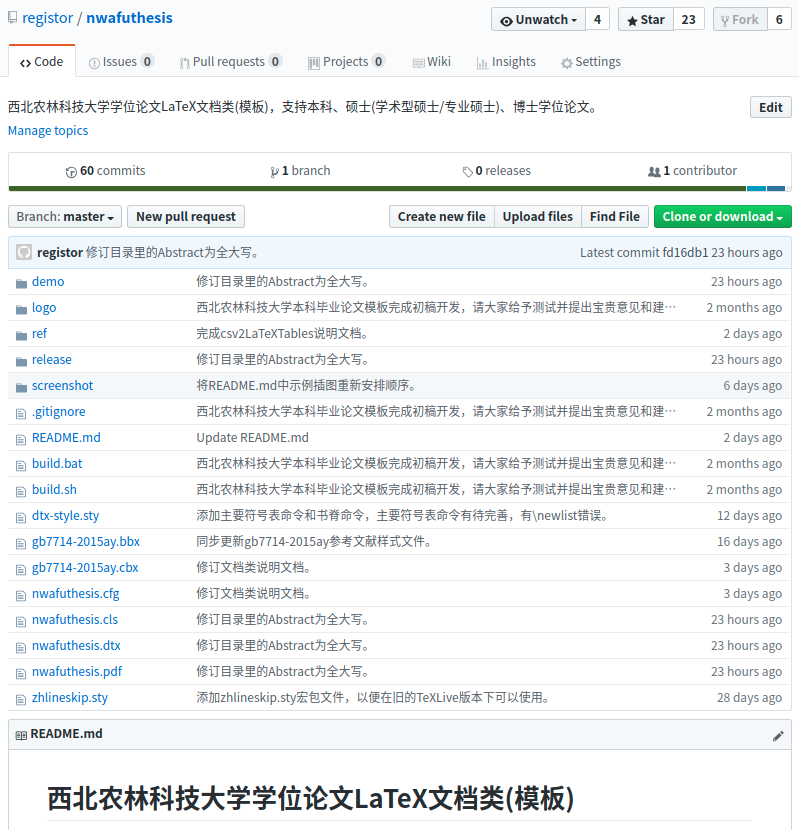
\includegraphics[height=0.6\textheight]{github}
  \stretchoff
\end{frame}

%%%%%%%%%%%%%%%%%%%%%%%%%%%%%% 关于我 %%%%%%%%%%%%%%%%%%%%%%%%%%%%%%%%%%%
\section[关于我]{关于我}
\subsection[联系方式]{联系方式}
\begin{frame}[fragile]{关于我}{联系方式}
  % colour options
  \definecolor{seplinecolour}{HTML}{357f2d} % green
  \definecolor{iconcolour}{HTML}{2f3142} % dark
  \definecolor{textcolour}{HTML}{2f3142} % dark
  \definecolor{jobtitlecolour}{HTML}{474a65} % light dark

  % define some lengths for internal spacing
  \newlength{\seplinewidth} \setlength{\seplinewidth}{2cm}
  \newlength{\seplineheight} \setlength{\seplineheight}{1pt}
  \newlength{\seplinedistance} \setlength{\seplinedistance}{0.3cm}
  \begin{center}
    \begin{tikzpicture}
      % name
      \matrix[every node/.style={anchor=center,font=\huge},anchor=center] (name) {
        \node{耿\hspace{\ccwd}楠}; \\
        %\node{Doe}; \\
        %\node{\color{jobtitlecolour}\normalsize\textit{教授}}; \\
      };
      % sep line 1
      \node[below=0.3\seplinedistance of name] (hl1) {};
      \draw[line width=\seplineheight,color=seplinecolour] (hl1)++(-\seplinewidth/2,0) -- ++(\seplinewidth,0);
      % contact info
      \matrix [below=\seplinedistance of hl1,%
               column 1/.style={anchor=center,color=iconcolour},%
               column 2/.style={anchor=west}] (contact) {
        \node{\faGlobe}; & \node{\url{http://cie.nwsuaf.edu.cn/szdw/js/}};\\
        \node{\faBuilding}; & \node{信息工程学院 317\texttt{\#}};\\ 
        \node{\faEnvelope}; & \node{nangeng@nwafu.edu.cn; nangeng@qq.com};\\
        %\node{\faQq}; & \node{970291228};\\
        %\node{\faPhone}; & \node{15829540966}; \\
        \node{\faGithub}; & \node{\url{https://github.com/registor/}}; \\
      };
      sep line 2
      \node[below=\seplinedistance of contact] (hl2) {};
      \draw[line width=\seplineheight,color=seplinecolour] (hl2)++(-\seplinewidth/2,0) -- ++(\seplinewidth,0);
      % interests
      \matrix [below=\seplinedistance of hl2,
         every node/.style={anchor=center,font=\LARGE}]
         (interests) {
        \node{\faCode}; & \node{\faCoffee}; &
        \node{\faLock}; & \node{\faWrench}; &
        \node{\faCameraRetro}; \\
      };
      
    \end{tikzpicture}
  \end{center}
\end{frame}

% 封底
%%%%%%%%%%%%%%%%

{
  \nwsuafwavesbg
  \begin{frame}[plain,noframenumbering]
    \finalpage{
      娟秀轻爽拉泰赫\\
      所写所想即所得\\
      排版何须穷思量\\
      窈窕俊俏尽婀娜\\
      \vspace{4ex}
      谢谢你使用该{\LaTeX} 简单教程!\\
      欢迎多提宝贵意见和建议}
  \end{frame}
}
%%%%%%%%%%%%%%%%
\end{document}

%%% Local Variables:
%%% mode: latex
%%% TeX-master: t
%%% End:
